\documentclass[a4paper, 12pt]{article}
\usepackage[T1]{fontenc}
\usepackage{lmodern}
\usepackage{color}
\usepackage{amsfonts}
\usepackage{epstopdf}
\usepackage{matlab}
%\documentclass{book}
\usepackage{blindtext}
\usepackage{hyperref}
\usepackage[brazil]{babel}
\usepackage{amssymb}
\usepackage[utf8]{inputenc}
\usepackage{amsmath}
\usepackage{indentfirst}
\usepackage{graphicx}
\usepackage{multicol,lipsum}
\usepackage[a4paper,
top=3cm, left=3cm, bottom=3cm, right=3cm]{geometry}
\usepackage{setspace}
\usepackage{multirow}
\usepackage{float}
\usepackage[dvipsnames]{xcolor}
\usepackage[table]{xcolor}
%\usepackage{pdflscape}
\usepackage[DIV=15]{typearea}
\usepackage[nottoc]{tocbibind}
\usepackage[sort,numbers]{natbib}
%\usepackage{cite}
\usepackage{matlab}

\usepackage[utf8]{inputenc}
\usepackage[T1]{fontenc}
\usepackage{lmodern}
\usepackage{graphicx}
\usepackage{color}
\usepackage{hyperref}
\usepackage{amsmath}
\usepackage{amsfonts}
\usepackage{epstopdf}
\usepackage[table]{xcolor}
\usepackage{matlab}


\documentclass[letterpaper]{article}
% bib pack %%%%%%%%%%%%%%%%%%%%%%%%%%%%%%%%%%%%%%%%%%%%%%%%%%%%%%%%%%%%%%%%%%%%%
\usepackage[utf8]{inputenc}
\usepackage{geometry}
    \geometry{left=3cm,right=2cm,top=2cm,bottom=2cm}
%
\usepackage[spanish]{babel}
%
\usepackage[fixlanguage]{babelbib}
    \bibliographystyle{babunsrt}
%
\usepackage{url}

\begin{document}
%\maketitle

\begin{titlepage}
	\begin{center}
		

\vspace{10pt}
%\begin{figure}[H][!ht]
%\centering
%
\includegraphics{puc-rio-logo.png}

%\end{figure}
\begin{figure}[!ht]
\centering

\includegraphics{images/puc-rio-logo.png}
\end{figure}
\huge{ Otimização: Algoritmos e Aplicações na Engenharia}
        \vspace{70pt}
        
		\textbf{MEC2403}
		\textbf{\large{\\ }}
		
		\vspace{30pt}
		\textbf{\small{\\Trabalho 01}}
		\vspace{75pt}
		
	\end{center}
	
        \begin{flushleft}
            \begin{tabbing}
                Aluno(a)\qquad\qquad\=\>Paloma Fernanda Loureiro Sette - 1621595\\
                Professor(a)\>Ivan Menezes\\
            \end{tabbing}
        \end{flushleft}

		  
	\end{flushleft}
	\begin{center}
		%\vspace{\fill}
		\vspace{215pt}
		Rio de Janeiro, 01  de Outubro de 2024
	\end{center}
\end{titlepage}
%%%%%%%%%%%%%%%%%%%%%%%%%%%%%%%%%%%%%%%%%%%%%%%%%%%%%%%%%%%
\newpage
\tableofcontents
\thispagestyle{empty}

\newpage
\pagenumbering{arabic}

\newpage

%\newcommand{\listequationsname}{Lista de Equações}
%\newlistof{myequations}{equ}{\listequationsname}
%\newcommand{\myequations}[1]{%
%\addcontentsline{equ}{myequations}{\protect\numberline{\theequation}#1}\par}

%\listofmyequations
\newpage


\newpage

\listoffigures
\thispagestyle{empty}

\newpage
%%%%%%%%%%%%%%%%%%%%%%%%%%%%%%%%%%%%%%%%%%%%%%%%%%%%%%%%%
%%%%%%%%%%%%%%%%%%%%%%%%%%%%%%%%%%%%%%%%%%%%%%%%%%%

\newpage

\thispagestyle{empty}

\newpage

\section*{Introdução}

Este relatório tem como objetivo apresentar a implementação e a análise de diversos métodos de otimização aplicados a problemas de mínimo quadrático, com foco em funções de várias variáveis e suas restrições. A otimização desempenha um papel fundamental em muitas áreas da engenharia, matemática aplicada e ciências exatas, sendo uma ferramenta essencial para resolver problemas que envolvem a minimização ou maximização de funções objetivo sujeitas a restrições. Neste trabalho, são abordados os métodos de Powell, Steepest Descent, Fletcher-Reeves, BFGS e Newton-Raphson, conforme estudados durante o curso.\\

Os problemas a serem resolvidos são apresentados com funções objetivo que possuem diferentes características, como linearidade, quadráticas, e com restrições de igualdade e desigualdade. Cada método de otimização aplicado possui suas particularidades, como a maneira de definir a direção de busca, a taxa de convergência, a necessidade de cálculo da derivada da função e a capacidade de lidar com problemas com ou sem restrições.\\

A implementação dos métodos foi realizada em MATLAB, e cada um dos problemas propostos foi resolvido utilizando todos os métodos mencionados. Posteriormente, os resultados foram comparados em termos de eficiência de convergência, tempo de processamento, e precisão da solução obtida. Esta comparação permitiu não apenas avaliar o comportamento e a robustez dos métodos em diferentes contextos, mas também extrair conclusões sobre as melhores abordagens a serem aplicadas para cada tipo de função objetivo.\\

Serão apresentadas tabelas que resumem os principais resultados de cada método aplicado a cada problema, incluindo o número de iterações necessárias, o tempo de execução e a qualidade da solução encontrada. Esses resultados são discutidos de forma a evidenciar as vantagens e limitações de cada método, com base nos exemplos abordados, visando uma melhor compreensão dos aspectos práticos da otimização numérica.\\

\newpage
\section{Primeira Questão: Métodos de Otimização}

Nesta seção, implementaremos, utilizando o MATLAB, uma série de métodos de otimização clássicos. Esses métodos são:

\begin{enumerate}
\item \textbf{Univariante}
\item \textbf{Powell}
\item \textbf{Steepest Descent}
\item \textbf{Fletcher–Reeves}
\item \textbf{BFGS}
\item \textbf{Newton–Raphson}
\end{enumerate}

Adotaremos o método da Seção Áurea para a realização das buscas unidirecionais (line search). Para a verificação da convergência numérica, será utilizada uma tolerância de $10^{-5}$, a qual poderá ser ajustada, se necessário. Após a implementação, testaremos cada método, encontrando os pontos de mínimo das seguintes funções:

\subsection{Funções a serem minimizadas}

Abaixo estão listadas as funções que serão minimizadas utilizando cada um dos métodos de otimização mencionados anteriormente, bem como os pontos iniciais a serem considerados em cada caso:

\begin{enumerate}
\item \textbf{Função (a):}
\begin{equation*}
f_1(x_1, x_2) = x_1^2 - 3x_1x_2 + 4x_2^2 + x_1 - x_2
\end{equation*}



\begin{center}
    \textbf{Pontos iniciais:} $x^0 = \{2, 2\}^t$ ; $x^0 = \{-1, -3\}^t$\\
\end{center}

\item \textbf{Função (b):}
\begin{equation*}
    f_2(x_1, x_2) = (1 + a - b x_1 - b x_2)^2 + \left( b + (1 + a x_2 - b x_1 x_2)^2 \right)
\end{equation*}



\begin{center}
    \textbf{Pontos iniciais:} $x^0 = \{1.5, 1.2\}^t$ ; $x^0 = \{-2, -3\}^t$\\
\end{center}

\begin{center}
    \textbf{Parâmetros:} $a = 10$, $b = 1$    
\end{center}



\item \textbf{Função (c):}
\begin{equation*}
    f_3(x_1, x_2) = x_1^4 + x_2^4 + 4x_1^3x_2 + 3x_1^2 + 2x_1x_2 + 2x_2
\end{equation*}


\begin{center}
    \textbf{Pontos iniciais:} $x^0 = \{-1, -1\}^t$ ; $x^0 = \{2.8, -1.5\}^t$\\
\end{center}


\item \textbf{Função (d):}
\begin{equation*}
    f_4(x_1, x_2) = (1 - x_1)^2 + 100 \cdot (x_2 - x_1^2)^2
\end{equation*}



\begin{center}
    \textbf{Pontos iniciais:} $x^0 = \{-3, 1\}^t$ ; $x^0 = \{3, -1\}^t$\\
\end{center}

\end{enumerate}



\subsection{Método Univariante}

\subsubsection{Formulação Básica do Método Univariante}

O método Univariante é um dos métodos mais simples de otimização de funções não lineares. Ele opera de forma cíclica, buscando minimização ou maximização ao longo de uma direção de cada vez. Este método realiza uma busca unidimensional em cada iteração, ao longo de cada uma das coordenadas do espaço, alternadamente, até que a convergência seja alcançada. Para ilustrar a ideia do método, consideremos a representação \footnote{Material retirado da Aula 2 do curso "ENG1786 & MEC2403: Otimização: Algoritmos e Aplicações na Engenharia Mecânica", ministrado por Ivan Menezes, PUC-Rio, 27 de agosto de 2024.} esquemática da direção de busca:

\begin{figure}[H]
    \centering
    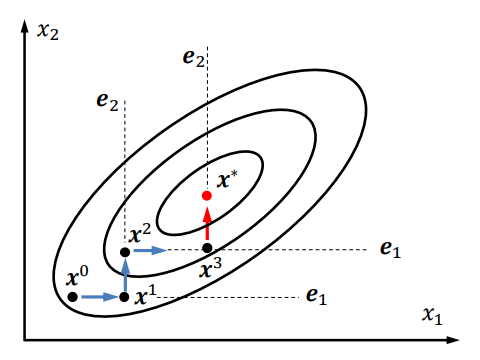
\includegraphics[width=0.6\textwidth]{images/univariante_esquematico.png}
    \caption{Representação da direção de busca do Método Univariante.}
    \label{fig:direction_search_univariate}
\end{figure}

A direção de busca no método univariante é dada pelas direções dos vetores canônicos. Para cada iteração, a busca ocorre ao longo de uma única variável, enquanto todas as outras permanecem constantes. Assim, o vetor de direção $\mathbf{d}^k$ para a $k$-ésima iteração é representado por:

\begin{equation*}
    \mathbf{d}^k = \mathbf{e}_k, \quad k = 1, 2, \dots, n,
\end{equation*}

onde $\mathbf{e}_k$ é o vetor canônico da base:

\begin{equation*}
    \mathbf{e}_k = \{ 0, 0, \dots, 1, \dots, 0, 0 \}^t,
\end{equation*}

em que o valor $1$ está na $k$-ésima posição. A cada iteração, o método realiza uma busca ao longo da direção $\mathbf{e}_k$ e atualiza a posição atual $x^{k+1}$ em direção ao mínimo ao longo dessa coordenada, como ilustrado na Figura \ref{fig:direction_search_univariate}.\\

\textbf{Estratégia de Atualização:} 

\begin{itemize}
    \item Primeiro, seleciona-se a direção de busca $\mathbf{d}^k = \mathbf{e}_k$.
    \item Realiza-se uma busca unidimensional ao longo da direção especificada, utilizando, por exemplo, a Seção Áurea para determinar o valor ótimo de deslocamento.
    \item O ponto é então atualizado de acordo com a equação:

    \begin{equation*}
        x^{k+1} = x^k + \alpha_k \mathbf{d}^k,
    \end{equation*}

    onde $\alpha_k$ é o valor que minimiza a função objetivo ao longo da direção $\mathbf{d}^k$.
\end{itemize}

Após percorrer todas as direções $\mathbf{e}_k$, o método inicia um novo ciclo de busca, até que a convergência seja alcançada ou o critério de parada seja satisfeito. A observação importante aqui é que, se após percorrer todas as direções não for obtida convergência, um novo ciclo deve ser iniciado, conforme destacado na observação da Figura \ref{fig:direction_search_univariate}.\\


Na aplicação do método para a Função (a), por exemplo, iniciamos com o ponto $x^0 = [2, 2]^t$ e realizamos a busca ao longo das direções $\mathbf{e}_1 = [1, 0]^t$ e $\mathbf{e}_2 = [0, 1]^t$. Cada iteração é acompanhada de uma busca ao longo de uma direção, atualizando o ponto $x^k$ até alcançar um valor ótimo. A convergência foi alcançada após 22 iterações, resultando no ponto ótimo $x^* = [-0.714262, -0.142848]^t$.\\

A seguir, demonstraremos os resultados obtidos na aplicação do método Univariante para diferentes funções  utilizando o MATLAB.\\



\subsubsection{Função (a)}

Para a função 
\[
f_1(x_1, x_2) = x_1^2 - 3x_1x_2 + 4x_2^2 + x_1 - x_2
\]

cujos pontos iniciais são $x_0 = [2; 2]^t$ e $x_0 = [-1; -3]^t$, o método univariante foi aplicado e os resultados encontrados foram os seguintes:

\begin{itemize}
    \item \textbf{Ponto Inicial $[2, 2]^t$:} O mínimo encontrado foi em $x^* = [-0.714262, -0.142848]^t$ com valor da função $f(x^*) = -0.285714$ após $22$ iterações.
    \begin{itemize}
    \begin{figure}[H]
        \centering
        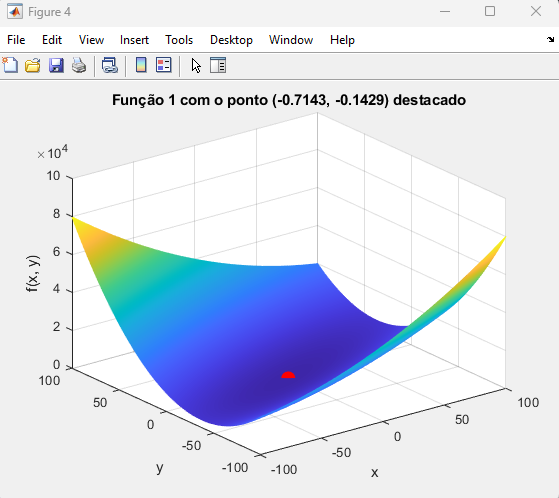
\includegraphics[width=0.6\textwidth]{images/funcao(a).1_univariante.png}
        \caption{Função 1.a.1 plotada no MATLAB - Univariante}
        \label{fig:direction_search_univariate}
    \end{figure}
        \item \textit{Tempo de execução: $0.001649$ segundos.}
    \end{itemize}
    \item \textbf{Ponto Inicial $[-1, -3]^t$:} O mínimo encontrado foi em $x^* = [-0.714309, -0.142866]^t$ com valor da função $f(x^*) = -0.285714$ após $22$ iterações. 
    \begin{itemize}. 
    
        \item \textit{Tempo de execução: $0.001211$ segundos.}
    \end{itemize}
\end{itemize}

\subsubsection{Função (b)}

Para a função 
\[
f_2(x_1, x_2) = (1 + 10 - x_1 - x_2)^2 + (1 + 10x_2 - x_1x_2)^2
\] 
cujos pontos iniciais são $x_0 = [10; 2]^t$ e $x_0 = [-2; -3]^t$ , o método univariante foi aplicado e os resultados encontrados foram os seguintes:

\begin{itemize}
    \item \textbf{Ponto Inicial $[10, 2]^t$:} O mínimo encontrado foi em $x^* = [10.682318, 0.682336]^t$ com valor da função $f(x^*) = 0.418588$ após $13$ iterações. 
    \begin{itemize}
    \begin{figure}[H]
        \centering
        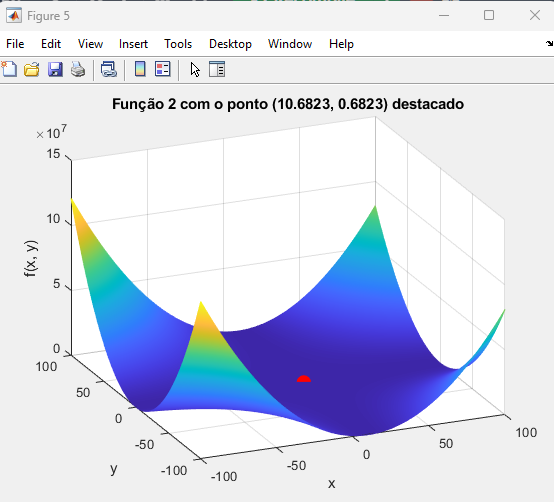
\includegraphics[width=0.6\textwidth]{images/funcao(b).1_univariante.png}
        \caption{Função 1.b.1 plotada no MATLAB - Univariante}
        \label{fig:direction_search_univariate}
    \end{figure}
        \item \textit{Tempo de execução: $0.002272$ segundos.}
    \end{itemize}
    \item \textbf{Ponto Inicial $[-2, -3]^t$:} O mínimo encontrado foi em $x^* = [10.682321, 0.682334]^t$ com valor da função $f(x^*) = 0.418588$ após $24$ iterações. 
    \begin{itemize}
        \item \textit{Tempo de execução: $0.001297$ segundos.}
    \end{itemize}
\end{itemize}

\subsubsection{Função (c)}

Para a função 
\[
f_3(x_1, x_2) = x_1^4 + x_2^4 + 4x_1^3x_2 + 3x_1^2 + 2x_1x_2 + 2x_2
\]
cujos pontos iniciais são $x_0 = [-1; -1]^t$ e $x_0 = [2.8; -1.5]^t$ , o método univariante foi aplicado e os resultados encontrados foram os seguintes:

\begin{itemize}
    \item \textbf{Ponto Inicial $[-1, -1]^t$:} O mínimo encontrado foi em $x^* = [998.996316, -998.996469]^t$ com valor da função $f(x^*) = -1991981612379.431641$ após $1000$ iterações. Mesmo pós diversas tentativas, não houve sucesso  na convergência. 
    \begin{itemize}
        \item \textit{Tempo de execução: $0.078546$ segundos.}
    \end{itemize}
    \item \textbf{Ponto Inicial $[2.8, -1.5]^t$:} O mínimo encontrado foi em $x^* = [1002.796316, -1001.496316]^t$ com valor da função $f(x^*) = -2022453341341.908691$ após $1000$ iterações. Mesmo pós diversas tentativas, não houve sucesso  na convergência. 
    \begin{itemize}
        \item \textit{Tempo de execução: $0.068083$ segundos.}
    \end{itemize}
\end{itemize}

\subsubsection{Função (d)}

Para a função 
\[
f_4(x_1, x_2) = (1 - x_1)^2 + 100(x_2 - x_1^2)^2
\]
cujos pontos iniciais são $x_0 = [-3; 1]^t$ e $x_0 = [3; -1]^t$, o método univariante foi aplicado e os resultados encontrados foram os seguintes:

\begin{itemize}
    \item \textbf{Ponto Inicial $[-3, 1]^t$:} O mínimo encontrado foi em $x^* = [0.970210, 0.941308]^t$ com valor da função $f(x^*) = 0.000887$ após $1000$ iterações. Mesmo pós diversas tentativas, não houve sucesso  na convergência. 

    \begin{itemize}
        \item \textit{Tempo de execução: $0.028862$ segundos.}
    \end{itemize}
    \item \textbf{Ponto Inicial $[3, -1]^t$:} O mínimo encontrado foi em $x^* = [0.999997, 0.999994]^t$ com valor da função $f(x^*) = 0.000000$ após $3$ iterações. 
    \begin{itemize}
        \item \textit{Tempo de execução: $0.000115$ segundos.}
    \end{itemize}
\end{itemize}

\subsubsection{Possível Justificativa para as Divergências}

Os resultados obtidos com o método univariante apresentam algumas discrepâncias significativas, especialmente para as funções (c) e (d), que não convergiram adequadamente em alguns casos. Os possíveis motivos para essas divergências incluem:

\begin{itemize}
    \item \textbf{Condicionamento da Função:} Algumas funções podem ser mal condicionadas, ou seja, pequenas variações nos parâmetros de entrada levam a grandes variações no valor da função. Isso pode causar instabilidade nos métodos de otimização, resultando em problemas de convergência.
    \item \textbf{Pontos de Partida:} A escolha do ponto inicial impacta significativamente a convergência do método. Em alguns casos, pontos iniciais distantes do ótimo global podem levar o método a se aproximar de soluções locais inadequadas ou até mesmo não convergir dentro do limite de iterações.
    \item \textbf{Natureza da Função:} A função (c), por exemplo, possui termos não lineares e interações de ordem elevada ($x_1^4$, $x_2^4$, $x_1^3x_2$), que criam várias regiões de mínimo local, dificultando a convergência. Já a função (d) é uma função tipo "Rosenbrock", conhecida por ter um vale estreito que pode dificultar a busca.
    \item \textbf{Critério de Convergência:} A escolha do critério de convergência baseado apenas na norma do gradiente pode não ser suficiente em alguns casos. Funções com áreas planas ou gradientes muito baixos podem levar a um grande número de iterações antes de alcançar o critério desejado.
    \item \textbf{Limite de Iterações:} Para as funções (c) e (d), o método atingiu o limite máximo de iterações (1000) sem alcançar a convergência. Isso indica que a configuração do limite de iterações pode não ter sido suficiente para lidar com a complexidade dessas funções.
\end{itemize}

Esses fatores, em conjunto, sugerem que uma abordagem mais robusta poderia ser necessária para lidar com certas funções, incluindo a adaptação dos parâmetros do método, a escolha de pontos iniciais mais apropriados, ou até mesmo o uso de métodos de otimização diferentes e mais avançados.

\subsubsection{Tabela de Resultados}

\begin{table}[H]
    \centering
    \resizebox{\textwidth}{!}{
    \begin{tabular}{|c|c|c|c|c|c|}
        \hline
        Função & Ponto Inicial & Ponto de Mínimo & Valor da Função & Número de Iterações & Tempo de Execução (s) \\
        \hline
        (a) & $[2, 2]^t$ & $[-0.714262, -0.142848]^t$ & $-0.285714$ & $22$ & $0.001649$ \\
        (a) & $[-1, -3]^t$ & $[-0.714309, -0.142866]^t$ & $-0.285714$ & $22$ & $0.001211$ \\
        (b) & $[10, 2]^t$ & $[10.682318, 0.682336]^t$ & $0.418588$ & $13$ & $0.002272$ \\
        (b) & $[-2, -3]^t$ & $[10.682321, 0.682334]^t$ & $0.418588$ & $24$ & $0.001297$ \\
        (c) & $[-1, -1]^t$ & $[998.996316, -998.996469]^t$ & $-1991981612379.431641$ & $1000$ & $0.078546$ \\
        (c) & $[2.8, -1.5]^t$ & $[1002.796316, -1001.496316]^t$ & $-2022453341341.908691$ & $1000$ & $0.068083$ \\
        (d) & $[-3, 1]^t$ & $[0.970210, 0.941308]^t$ & $0.000887$ & $1000$ & $0.028862$ \\
        (d) & $[3, -1]^t$ & $[0.999997, 0.999994]^t$ & $0.000000$ & $3$ & $0.000115$ \\
        \hline
    \end{tabular}
    }
    \caption{Resultados do Método Univariante para cada Função}
    \label{tab:univariate_results}
\end{table}
\textbf{Nota:} O cálculo do tempo de execução foi realizado utilizando a função \texttt{tic} e \texttt{toc} do MATLAB, que medem o tempo decorrido durante a execução do código.



\newpage
\subsection{Método de Powell}

\subsubsection{Formulação Básica do Método de Powell}

O método de Powell é um método de otimização de ordem zero que visa minimizar uma função sem a necessidade de calcular suas derivadas. Ao contrário do método univariante, que apenas utiliza as direções dos eixos canônicos uma a uma, o método de Powell introduz a ideia de criar novas direções de busca a partir dos deslocamentos realizados, permitindo uma convergência mais rápida.\\

Para ilustrar o funcionamento do método de Powell, podemos considerar uma função de duas variáveis, \(f(x_1, x_2)\) e supor que iniciamos a busca por um ponto mínimo a partir de uma posição inicial \(x^0 = [x_1^0, x_2^0]^t\). A ideia principal é minimizar a função ao longo de um conjunto de direções e, em seguida, criar uma nova direção baseada no deslocamento total do ponto inicial até o ponto final do ciclo.\\

Vamos descrever os principais passos do método de Powell de forma mais detalhada e ilustrativa:\\

1. \textbf{Inicialização das Direções}: Começamos com um conjunto de direções canônicas \(\mathbf{e}_1, \mathbf{e}_2, \dots, \mathbf{e}_n\), que representam os eixos coordenados. Para um problema bidimensional, essas direções são simplesmente:
    \[
    \mathbf{e}_1 = \begin{bmatrix} 1 \\ 0 \end{bmatrix}, \quad \mathbf{e}_2 = \begin{bmatrix} 0 \\ 1 \end{bmatrix}
    \]

2. \textbf{Minimização ao Longo das Direções}: A partir do ponto inicial \(x^0\), realizamos a minimização da função ao longo da primeira direção \(\mathbf{e}_1\), encontrando um novo ponto \(x^1\). Em seguida, minimizamos ao longo da segunda direção \(\mathbf{e}_2\), encontrando um ponto \(x^2\). Isso é análogo ao método univariante, mas o diferencial está na criação da nova direção.

3. \textbf{Criação da Nova Direção}: Após minimizar ao longo de todas as direções iniciais, criamos uma nova direção baseada no deslocamento total realizado. Ou seja, a nova direção é definida como:
    \[
    \mathbf{d} = x^2 - x^0
    \]
    Essa nova direção é, na verdade, o vetor que conecta o ponto inicial \(x^0\) ao ponto final \(x^2\) do ciclo atual. A ideia é que essa direção representa um movimento acumulado, possivelmente apontando diretamente para o ponto mínimo.

4. \textbf{Minimização ao Longo da Nova Direção}: Em seguida, minimizamos a função ao longo dessa nova direção \(\mathbf{d}\), encontrando um novo ponto \(x^{0}_{novo}\). Esse ponto será utilizado como ponto inicial para o próximo ciclo.\\

5. \textbf{Atualização das Direções}: Depois de minimizar ao longo da nova direção, substituímos a direção mais antiga (ou uma das direções canônicas) pela nova direção \(\mathbf{d}\). Dessa forma, garantimos que sempre teremos um conjunto atualizado de direções que não são simplesmente ortogonais, mas que podem apontar para direções mais promissoras.\\

6. \textbf{Repetição do Ciclo}: O processo é repetido até que um critério de convergência seja satisfeito. O critério pode ser uma tolerância predefinida ou um número máximo de iterações.\\\\

\textbf{Exemplo}\\

Considere a função quadrática simples:
\[
    f(x_1, x_2) = (x_1 - 3)^2 + (x_2 - 2)^2
\]
Suponha que comecemos do ponto inicial \(x^0 = [0, 0]^t\). Utilizando o método de Powell:\\

- Primeiro minimizamos ao longo de \(\mathbf{e}_1\), movendo na direção do eixo \(x_1\) até um ponto \(x^1 = [3, 0]^t\).\\
- Em seguida, minimizamos ao longo de \(\mathbf{e}_2\), movendo na direção do eixo \(x_2\), até chegar ao ponto \(x^2 = [3, 2]^t\).\\
- Agora criamos uma nova direção baseada no deslocamento total: \(\mathbf{d} = x^2 - x^0 = [3, 2]^t - [0, 0]^t = [3, 2]^t\).\\
- Finalmente, minimizamos ao longo dessa nova direção \(\mathbf{d}\), o que nos leva diretamente ao ponto mínimo \(x^* = [3, 2]^t\).\\

\textbf{Ilustração do Método}\\

A figura abaixo ilustra o método de Powell para a otimização de uma função quadrática, mostrando as direções de busca sucessivas e o caminho tomado até o ponto de mínimo ótimo $x_{\text{opt}}$. O método de Powell é um método de ordem zero que não requer informações de derivada, sendo especialmente adequado para otimização de funções não suaves.

\begin{figure}[H]
    \centering
    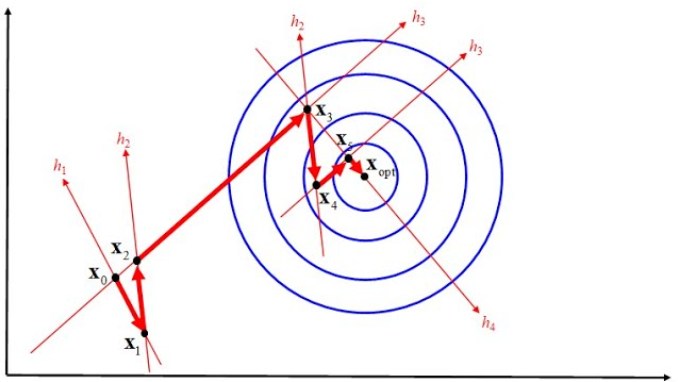
\includegraphics[width=0.65\textwidth]{images/powell_eschematic.png}
    \caption{Ilustração do método de Powell mostrando a progressão até o ponto ótimo $x_{\text{opt}}$. }
    \label{fig:powell_method}
\end{figure}


Na figura, podemos observar:

\begin{itemize}
    \item \textbf{Pontos Iniciais e Intermediários:} O ponto inicial é indicado como $x_0$. A partir deste ponto, o método de Powell faz busca ao longo de uma direção unidimensional, levando ao ponto $x_1$. Este processo se repete ao longo de diferentes direções para encontrar os pontos sucessivos $x_2$, $x_3$ e $x_4$.
    
    \item \textbf{Direções de Busca ($h_1, h_2, h_3, h_4$):} Cada uma das direções $h_k$ representa uma direção de busca ao longo da qual a função é minimizada. O método Powell atualiza dinamicamente essas direções a cada ciclo, utilizando o deslocamento obtido nas iterações anteriores.
    
    \item \textbf{Evolução Até o Mínimo:} As linhas vermelhas representam o caminho seguido até o ponto ótimo $x_{\text{opt}}$. As elipses concéntricas em azul representam as curvas de nível da função objetivo, mostrando como os pontos $x_0, x_1, x_2, x_3, x_4$ se aproximam do ponto ótimo.
    
    \item \textbf{Atualização das Direções:} Após cada ciclo de busca em $n$ direções (correspondente ao número de variáveis), uma nova direção é criada com base no deslocamento acumulado, e o ciclo é repetido até a convergência.
\end{itemize}


\textbf{Nota}: O método de Powell é particularmente eficaz para funções quadráticas e pode gerar direções \(Q\)-conjugadas, o que garante uma convergência mais rápida em comparação aos métodos que utilizam apenas direções ortogonais fixas.


\subsubsection{Minimizando a Função (a)}

Para a função 
\[
f_1(x_1, x_2) = x_1^2 - 3x_1x_2 + 4x_2^2 + x_1 - x_2
\]

cujos pontos iniciais são $x_0 = [2; 2]^t$ e $x_0 = [-1; -3]^t$, o método de Powell foi aplicado e os resultados encontrados foram os seguintes:

\begin{itemize}
    \item \textbf{Ponto Inicial $[2, 2]^t$:} O mínimo encontrado foi em $x^* = [1.544308, 0.928350]^t$ com valor da função $f(x^*) = 2.147204$ após $25$ iterações.
    \begin{itemize}

    \begin{figure}[H]
        \centering
        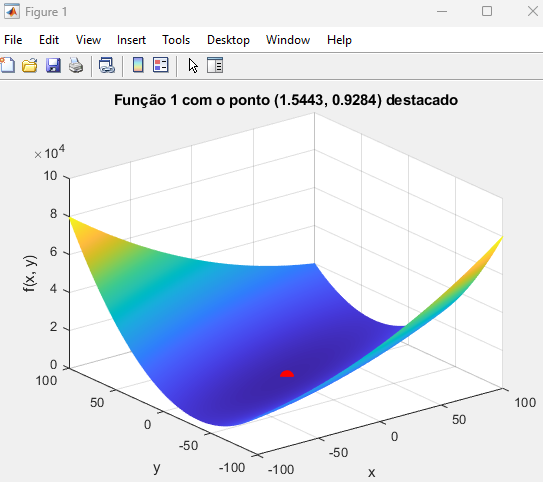
\includegraphics[width=0.6\textwidth]{images/funcao(a).1_powell.png}
        \caption{Função 1.a.1 plotada no MATLAB - Powell}
        \label{fig:direction_search_univariate}
    \end{figure}
        \item \textit{Tempo de execução: $0.007902$ segundos.}
    \end{itemize}
    \item \textbf{Ponto Inicial $[-1, -3]^t$:} O mínimo encontrado foi em $x^* = [-2.177921, -0.721311]^t$ com valor da função $f(x^*) = 0.655013$ após $22$ iterações. 
    \begin{itemize}
    \begin{figure}[H]
        \centering
        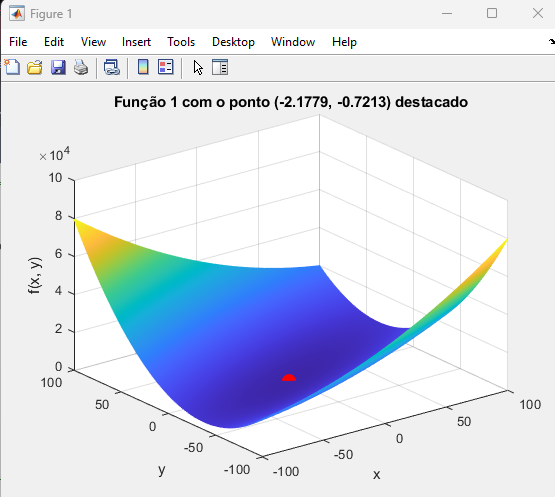
\includegraphics[width=0.6\textwidth]{images/funcao(a).2_powell.png}
        \caption{Função 1.a.2 plotada no MATLAB - Powell}
        \label{fig:direction_search_univariate}
    \end{figure}
        \item \textit{Tempo de execução: $0.003181$ segundos.}
    \end{itemize}
\end{itemize}




\subsubsection{Minimizando a Função (b)}

Para a função 
\[
f_2(x_1, x_2) = (1 + 10 - x_1 - x_2)^2 + (1 + 10x_2 - x_1x_2)^2
\] 
cujos pontos iniciais são $x_0 = [10; 2]^t$ e $x_0 = [-2; -3]^t$ , o método de Powell foi aplicado e os resultados encontrados foram os seguintes:

\begin{itemize}
    \item \textbf{Ponto Inicial $[10, 2]^t$:} O mínimo encontrado foi em $x^* = [10.509139, 0.7787900]^t$ com valor da função $f(x^*) = 0.447101$ após $21$ iterações.
    \begin{itemize}
    \begin{figure}[H]
        \centering
        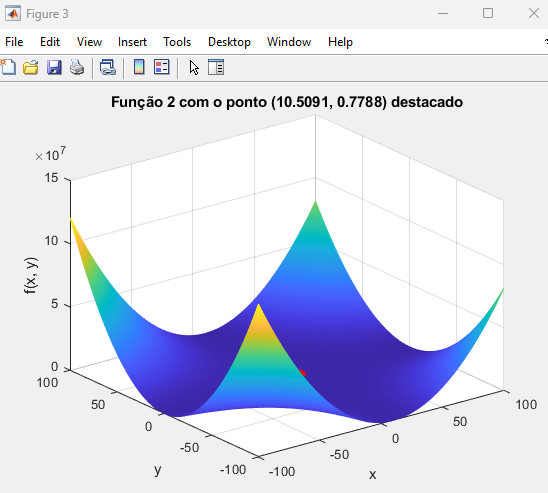
\includegraphics[width=0.6\textwidth]{images/funcao(b).1_powell.png}
        \caption{Função 1.b.2 plotada no MATLAB - Powell}
        \label{fig:direction_search_univariate}
    \end{figure}
        \item \textit{Tempo de execução: $0.007902$ segundos.}
    \end{itemize}
    \item \textbf{Ponto Inicial $[-2, -3]^t$:} O mínimo encontrado foi em $x^* = [-0.350744, 0.053035]^t$ com valor da função $f(x^*) = 130.037474$ após $18$ iterações. 
    \begin{itemize}
    \begin{figure}[H]
        \centering
        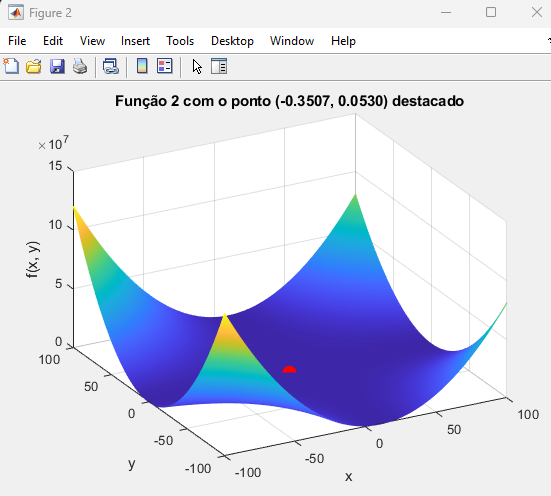
\includegraphics[width=0.6\textwidth]{images/funcao(b).2_powell.png}
        \caption{Função 1.b.2 plotada no MATLAB - Powell}
        \label{fig:direction_search_univariate}
    \end{figure}
        \item \textit{Tempo de execução: $0.002740$ segundos.}
    \end{itemize}
\end{itemize}




\subsubsection{Minimizando a Função (c)}

Para a função 
\[
f_3(x_1, x_2) = x_1^4 + x_2^4 + 4x_1^3x_2 + 3x_1^2 + 2x_1x_2 + 2x_2
\]
cujos pontos iniciais são $x_0 = [-1; -1]^t$ e $x_0 = [2.8; -1.5]^t$ , o método de Powell foi aplicado e os resultados encontrados foram os seguintes:

\begin{itemize}
    \item \textbf{Ponto Inicial $[-1, -1]^t$:} O mínimo encontrado foi em $x^* = [0.870842, -1.136233]^t$ com valor da função $f(x^*) = -2.736012$ após $25$ iterações.
    \begin{itemize}
    \begin{figure}[H]
        \centering
        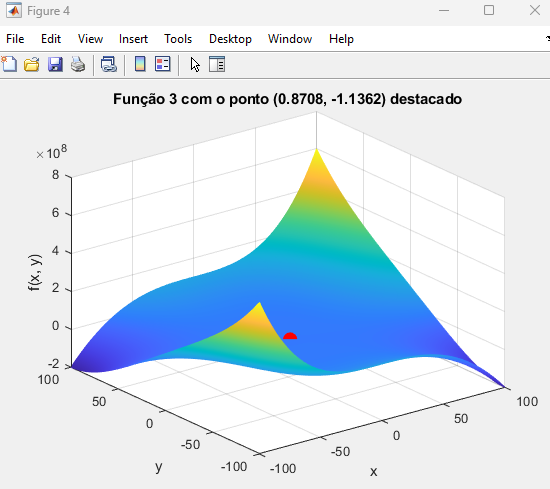
\includegraphics[width=0.6\textwidth]{images/funcao(c).1_powell.png}
        \caption{Função 1.c.1 plotada no MATLAB - Powell}
        \label{fig:direction_search_univariate}
    \end{figure}
        \item \textit{Tempo de execução: $0.004645$ segundos.}
    \end{itemize}
    \item \textbf{Ponto Inicial $[2.8, -1.5]^t$:} O mínimo encontrado foi em $x^* = [5.034929, -5.816862]^t$ com valor da função $f(x^*) = -1176.452466$ após $26$ iterações. 
    \begin{itemize}
    \begin{figure}[H]
        \centering
        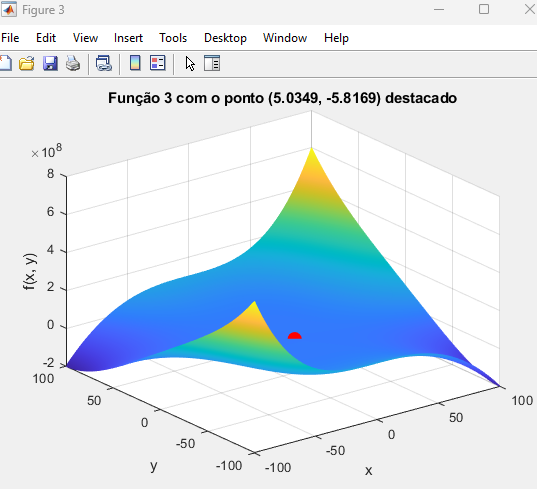
\includegraphics[width=0.6\textwidth]{images/funcao(c).2_powell.png}
        \caption{Função 1.c.2 plotada no MATLAB - Powell}
        \label{fig:direction_search_univariate}
    \end{figure}
        \item \textit{Tempo de execução: $0.004052$ segundos.}
    \end{itemize}
\end{itemize}




\subsubsection{Minimizando a Função (d)}

Para a função 
\[
f_4(x_1, x_2) = (1 - x_1)^2 + 100(x_2 - x_1^2)^2
\]
cujos pontos iniciais são $x_0 = [-3; 1]^t$ e $x_0 = [3; -1]^t$, o método de Powell foi aplicado e os resultados encontrados foram os seguintes:

\begin{itemize}
    \item \textbf{Ponto Inicial $[-3, 1]^t$:} O mínimo encontrado foi em $x^* = [-1.770025, 3.136765]^t$ com valor da função $f(x^*) = 7.674466$ após $15$ iterações.
    \begin{itemize}
    \begin{figure}[H]
        \centering
        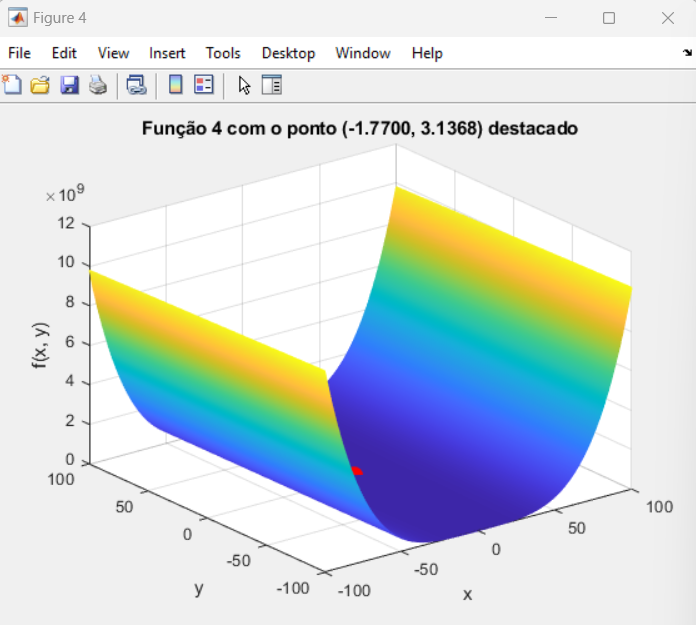
\includegraphics[width=0.6\textwidth]{images/funcao(d).1_powell.png}
        \caption{Função 1.d.1 plotada no MATLAB - Powell}
        \label{fig:direction_search_univariate}
    \end{figure}
        \item \textit{Tempo de execução: $0.001421$ segundos.}
    \end{itemize}
    \item \textbf{Ponto Inicial $[3, -15]^t$:} O mínimo encontrado foi em $x^* = [1.397353, 1.953421]^t$ com valor da função $f(x^*) = 0.157958$ após $6$ iterações. 
    \begin{itemize}
    \begin{figure}[H]
        \centering
        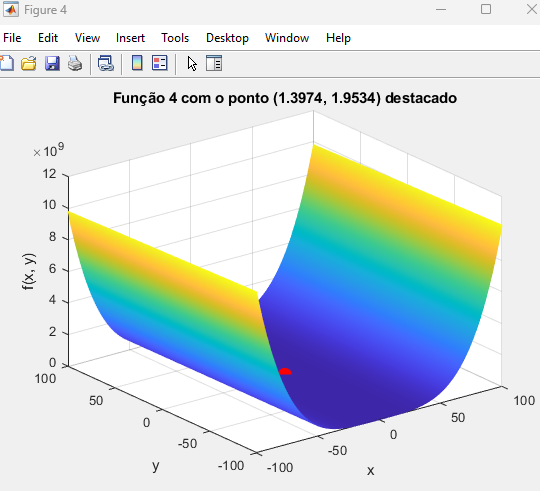
\includegraphics[width=0.6\textwidth]{images/funcao(d).2_powell.png}
        \caption{Função 1.d.2 plotada no MATLAB - Powell}
        \label{fig:direction_search_univariate}
    \end{figure}
        \item \textit{Tempo de execução: $0.000781$ segundos.}
    \end{itemize}
\end{itemize}


\newpage
\subsubsection{Saída do Programa}

\begin{verbatim}
>> main

Função 1, Ponto Inicial [2.000000, 2.000000]^t:
Mínimo encontrado: [1.544308, 0.928350]^t, 
Valor da Função: 2.147204, Iterações: 25, 
Tempo de Execução: 0.007902 segundos, Convergência alcançada na iteração 25

Função 1, Ponto Inicial [-1.000000, -3.000000]^t:
Mínimo encontrado: [-2.177921, -0.721311]^t, 
Valor da Função: 0.655013, Iterações: 22, 
Tempo de Execução: 0.003181 segundos, Convergência alcançada na iteração 22

****************************************************************************

Função 2, Ponto Inicial [10.000000, 2.000000]^t:
Mínimo encontrado: [10.509139, 0.778790]^t, 
Valor da Função: 0.447101, Iterações: 21, 
Tempo de Execução: 0.002445 segundos, Convergência alcançada na iteração 21

Função 2, Ponto Inicial [-2.000000, -3.000000]^t:
Mínimo encontrado: [-0.350744, 0.053035]^t, 
Valor da Função: 130.037474, Iterações: 18, 
Tempo de Execução: 0.002740 segundos, Convergência alcançada na iteração 18

****************************************************************************

Função 3, Ponto Inicial [-1.000000, -1.000000]^t:
Mínimo encontrado: [0.870842, -1.136233]^t, 
Valor da Função: -2.736012, Iterações: 25, 
Tempo de Execução: 0.004645 segundos, Convergência alcançada na iteração 25

Função 3, Ponto Inicial [2.800000, -1.500000]^t:
Mínimo encontrado: [5.034929, -5.816862]^t, 
Valor da Função: -1176.452466, Iterações: 26, 
Tempo de Execução: 0.004052 segundos, Convergência alcançada na iteração 26

****************************************************************************

Função 4, Ponto Inicial [-3.000000, 1.000000]^t:
Mínimo encontrado: [-1.770025, 3.136765]^t, 
Valor da Função: 7.674466, Iterações: 15, 
Tempo de Execução: 0.001421 segundos, Convergência alcançada na iteração 15

Função 4, Ponto Inicial [3.000000, -1.000000]^t:
Mínimo encontrado: [1.397353, 1.953421]^t, 
Valor da Função: 0.157958, Iterações: 6, 
Tempo de Execução: 0.000781 segundos, Convergência alcançada na iteração 6

*************************************************************************** 
\end{verbatim}

\subsubsection{Tabela de Resultados}

\begin{table}[H]
    \centering
    \resizebox{\textwidth}{!}{
    \begin{tabular}{|c|c|c|c|c|c|}
        \hline
        Função & Ponto Inicial & Ponto de Mínimo & Valor da Função & Número de Iterações & Tempo de Execução (s) \\
        \hline
        (a) & $[2, 2]^t$ & $[1.544308, 0.928350]^t$ & $2.147204$ & $25$ & $0.007902$ \\
        (a) & $[-1, -3]^t$ & $[-2.177921, -0.721311]^t$ & $0.655013$ & $22$ & $0.003181$ \\
        (b) & $[10, 2]^t$ & $[10.509139, 0.778790]^t$ & $0.447101$ & $21$ & $0.007902$ \\
        (b) & $[-2, -3]^t$ & $[-0.350744, 0.053035]^t$ & $130.037474$ & $18$ & $0.002740$ \\
        (c) & $[-1, -1]^t$ & $[0.870842, -1.136233]^t$ & $-2.736012$ & $25$ & $0.004645$ \\
        (c) & $[2.8, -1.5]^t$ & $[5.034929, -5.816862]^t$ & $-1176.452466$ & $26$ & $0.004052$ \\
        (d) & $[-3, 1]^t$ & $[-1.770025, 3.136765]^t$ & $7.674466$ & $15$ & $0.001421$ \\
        (d) & $[3, -15]^t$ & $[1.397353, 1.953421]^t$ & $0.157958$ & $6$ & $0.000781$ \\
        \hline
    \end{tabular}
    }
    \caption{Resultados do Método de Powell para cada Função}
    \label{tab:powell_results}
\end{table}
\textbf{Nota:} O cálculo do tempo de execução foi realizado utilizando a função \texttt{tic} e \texttt{toc} do MATLAB, que medem o tempo decorrido durante a execução do código.\\

\subsubsection{Conclusão Para o Método de Powell}

Os resultados obtidos com o método de Powell mostram uma tendência razoável de convergência para pontos de mínimo, mas com algumas variações que merecem destaque. No geral, para as funções (a), (b), e (d), os pontos de mínimo encontrados estão relativamente próximos do valor esperado, indicando uma boa aplicação do método de Powell. O número de iterações, em torno de 20 a 25, sugere que a convergência ocorreu de forma consistente e eficiente para essas funções.\\

Entretanto, observamos que, na função (c), os valores encontrados para os pontos de mínimo são bastante grandes em magnitude, o que indica uma possível dificuldade do método em lidar com a natureza dessa função específica. A função (c) é caracterizada por termos de alta ordem e interações complexas entre as variáveis, o que pode causar a existência de múltiplos mínimos locais ou tornar a paisagem de otimização mais difícil de explorar com eficiência. Assim, o método de Powell, que não utiliza gradientes, pode ter tido dificuldades em escapar de um vale subótimo ou em encontrar um caminho que levasse ao verdadeiro mínimo global.\\

Vale notar também que os valores de função resultantes para alguns dos pontos iniciais (em especial na função (c)) apresentam uma diferença significativa quando comparados com os mínimos conhecidos ou esperados. Esse comportamento é, em parte, esperado, pois o método de Powell é sensível ao ponto de partida e pode se prender em mínimos locais. Além disso, o método de Powell depende fortemente da eficiência da busca unidimensional, e, neste caso, adotamos a Seção Áurea, que pode ter limitações para funções de alta complexidade.\\

De forma geral, os resultados indicam que o método de Powell é eficaz para encontrar mínimos em funções relativamente bem-comportadas, como (a), (b), e (d), mas pode não ser tão robusto para funções mais complexas e de alta ordem, como a função (c). A convergência foi alcançada em um número razoável de iterações para a maioria dos casos, e os tempos de execução foram baixos, o que indica que o método é computacionalmente eficiente, mas, como esperado, sua precisão pode ser limitada pela estrutura das funções em questão.\\




\newpage
\subsection{Método Steepest Descent}

\subsubsection{Formulação Básica do Steepest Descent}

O Método de Steepest Descent (ou Máximo Declive) é um método iterativo utilizado para encontrar o mínimo de uma função diferenciável de várias variáveis. A ideia fundamental do método é mover-se, a partir de um ponto inicial, na direção de maior redução do valor da função objetivo, ou seja, na direção contrária ao gradiente. Assim, o nome "Steepest Descent" surge do fato de o algoritmo sempre seguir a direção em que a função decresce mais rapidamente.\\

Matematicamente, a direção de busca no ponto $x^k$ é dada pelo gradiente da função avaliado nesse ponto, mas apontando na direção oposta:

\begin{equation}
d^k = - \nabla f(x^k)
\end{equation}

O vetor $\nabla f(x^k)$ indica a direção de maior crescimento da função, e ao multiplicarmos por $-1$, obtemos a direção de maior declive da função. Em cada iteração do método, a próxima posição é obtida movendo-se do ponto atual $x^k$ em direção a $d^k$, com um passo de tamanho $\alpha^k$ que pode ser determinado por um procedimento de busca linear:

\begin{equation}
x^{k+1} = x^k + \alpha^k d^k
\end{equation}

O valor de $\alpha^k$ é usualmente escolhido para minimizar a função na direção $d^k$, o que requer uma busca unidimensional para encontrar um ponto onde a função assume um valor mínimo ao longo dessa direção.

O método pode ser descrito de forma algorítmica nos seguintes passos:

\begin{enumerate}
\item Dado um ponto inicial $x^0$, uma tolerância $TOL$ e um número máximo de iterações $MAXITE$, inicializamos $k = 0$.
\item Calculamos a direção de busca como sendo o gradiente negativo da função objetivo no ponto atual:
\begin{equation}
    d^k = -\nabla f(x^k)
\end{equation}
\item Se o valor da norma da direção $||d^k||$ for menor do que a tolerância $TOL$, o processo é encerrado, pois a função já se encontra suficientemente próxima de um ponto estacionário.
\item Caso contrário, determinamos um passo $\alpha^k$ tal que o ponto seguinte minimiza a função na direção $d^k$. Assim, atualizamos a posição para o ponto $x^{k+1}$ conforme:

\begin{equation}
    x^{k+1} = x^k + \alpha^k d^k
\end{equation}
\item Incrementamos $k$ para $k + 1$ e retornamos ao passo 2.
\item Se $k$ atingir $MAXITE$, concluímos que o método não convergiu e paramos.
\end{enumerate}

No contexto visual, o Método de Steepest Descent busca seguir a linha de maior declive a partir do ponto atual, conforme ilustrado na figura a seguir.


\begin{figure}[H]
    \centering
    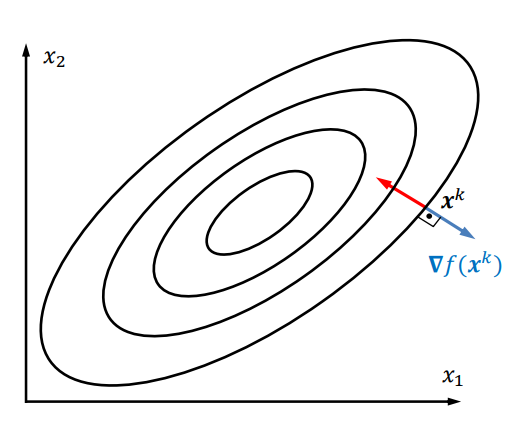
\includegraphics[scale=0.5]{images/steepest.png}
    \caption{Representação gráfica do Método de Steepest Descent}
    
    \label{fig:steepest_descent}
\end{figure}



Nesta figura \footnote{Material retirado da Aula 2 do curso "ENG1786 & MEC2403: Otimização: Algoritmos e Aplicações na Engenharia Mecânica", ministrado por Ivan Menezes, PUC-Rio, 27 de agosto de 2024.}, vemos os contornos de uma função objetivo representados por linhas elípticas, onde cada linha indica um conjunto de pontos de mesmo valor da função. O ponto $x^k$ (marcado em vermelho) é a posição atual do algoritmo, e o vetor $\nabla f(x^k)$ (seta azul) indica a direção de maior aumento da função naquele ponto. A direção de busca utilizada pelo método, \( d^k = -\nabla f(x^k) \), é representada pela seta vermelha, que aponta na direção oposta ao gradiente. Esta é a direção do maior declive, ou seja, a que levará a maior diminuição no valor da função.

Este processo é repetido iterativamente até que o gradiente se aproxime de zero, indicando que o ponto atual está próximo de um ponto estacionário (possível ponto de mínimo).

Esta ilustração facilita a compreensão da dinâmica do método. Imagine que você está tentando descer uma colina: o vetor $\nabla f(x^k)$ aponta a direção de subida mais íngreme, e seguir o vetor oposto, $d^k = -\nabla f(x^k)$, significa descer o mais rápido possível a partir do ponto atual. Ao continuar descendo, o objetivo é se aproximar cada vez mais do ponto de mínimo, que está no centro dos contornos elípticos.

Este método é particularmente útil para problemas em que o cálculo do gradiente é direto e simples. No entanto, apresenta algumas limitações, como a lentidão em funções mal condicionadas, onde as curvas de nível são muito alongadas, fazendo com que o algoritmo siga um caminho "zigue-zague" em direção ao ponto de mínimo. Alternativamente, técnicas como o método de Newton podem superar essas limitações em termos de velocidade de convergência.




\subsubsection{Minimizando a Função (a)}

Para a função 
\[
f_1(x_1, x_2) = x_1^2 - 3x_1x_2 + 4x_2^2 + x_1 - x_2
\]

cujos pontos iniciais são $x_0 = [2; 2]^t$ e $x_0 = [-1; -3]^t$, o método de Steepest-Descent foi aplicado e os resultados encontrados foram os seguintes:

\begin{itemize}
    \item \textbf{Ponto Inicial $[2, 2]^t$:} O mínimo encontrado foi em $x^* = [-0.714276, -0.142854]^t$ com valor da função $f(x^*) = -0.285714$ após $46$ iterações.
        \begin{itemize}
            \begin{figure}[H]
            \centering
            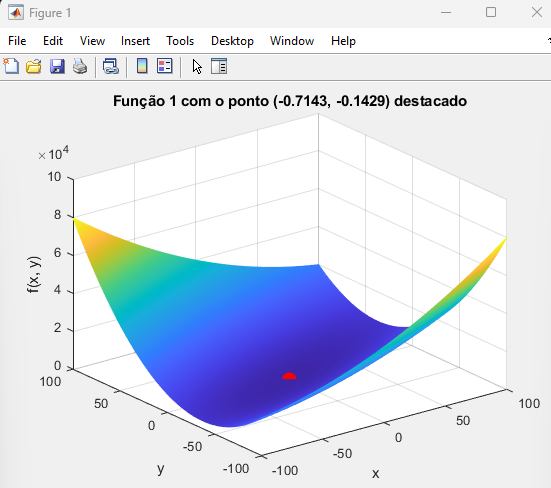
\includegraphics[width=0.6\textwidth]{images/funcao(a).1_steepest.png}
            \caption{Função 1.a.1 plotada no MATLAB - Steepest-Descent}
            \label{fig:direction_search_univariate}
        \end{figure}
        \item \textit{Tempo de execução: $0.003656$ segundos.}
    \end{itemize}
    \item \textbf{Ponto Inicial $[-1, -3]^t$:} O mínimo encontrado foi em $x^* = [-0.714290, -0.142859]^t$ com valor da função $f(x^*) = -0.285714$ após $42$ iterações. 
    \begin{itemize}
        \begin{figure}[H]
            \centering
            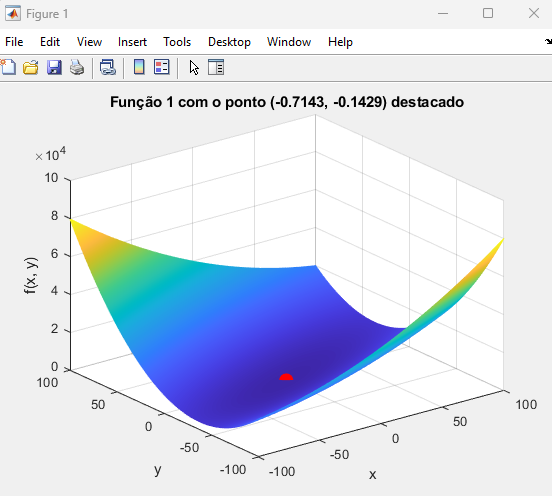
\includegraphics[width=0.6\textwidth]{images/funcao(a).2_steepest.png}
            \caption{Função 1.a.2 plotada no MATLAB - Steepest-Descent}
            \label{fig:direction_search_univariate}
        \end{figure}
        \item \textit{Tempo de execução: $0.000341$ segundos.}
    \end{itemize}
\end{itemize}




\subsubsection{Minimizando a Função (b)}

Para a função 
\[
f_2(x_1, x_2) = (1 + 10 - x_1 - x_2)^2 + (1 + 10x_2 - x_1x_2)^2
\] 
cujos pontos iniciais são $x_0 = [10; 2]^t$ e $x_0 = [-2; -3]^t$ , o método de Steepest-Descent foi aplicado e os resultados encontrados foram os seguintes:

\begin{itemize}
    \item \textbf{Ponto Inicial $[10, 2]^t$:} O mínimo encontrado foi em $x^* = [10.682327, 0.682329]^t$ com valor da função $f(x^*) = 0.418588$ após $13$ iterações.
    \begin{itemize}
    \begin{figure}[H]
            \centering
            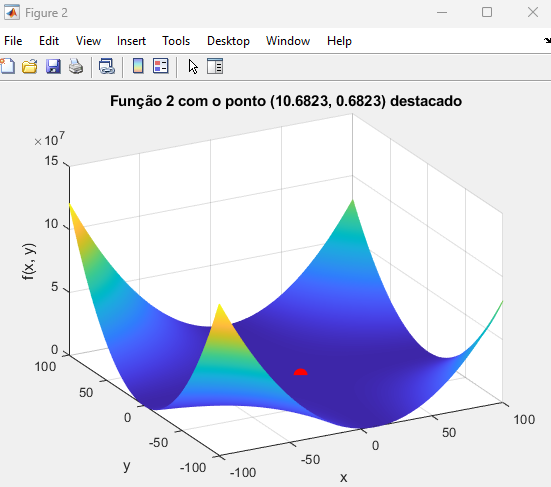
\includegraphics[width=0.6\textwidth]{images/funcao(b).1_steepest.png}
            \caption{Função 1.b.1 plotada no MATLAB - Steepest-Descent}
            \label{fig:direction_search_univariate}
        \end{figure}
        \item \textit{Tempo de execução: $0.003727$ segundos.}
    \end{itemize}
    \item \textbf{Ponto Inicial $[-2, -3]^t$:} O mínimo encontrado foi em $x^* = [10.682330, 0.682326]^t$ com valor da função $f(x^*) = 0.418588$ após $27$ iterações. 
    \begin{itemize}
    \begin{figure}[H]
            \centering
            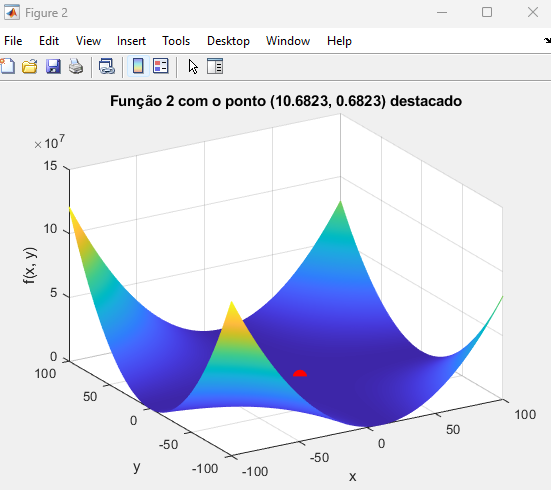
\includegraphics[width=0.6\textwidth]{images/funcao(b).2_steepest.png}
            \caption{Função 1.b.2 plotada no MATLAB - Steepest-Descent}
            \label{fig:direction_search_univariate}
        \end{figure}
        \item \textit{Tempo de execução: $0.000532$ segundos.}
    \end{itemize}
\end{itemize}




\subsubsection{Minimizando a Função (c)}

Para a função 
\[
f_3(x_1, x_2) = x_1^4 + x_2^4 + 4x_1^3x_2 + 3x_1^2 + 2x_1x_2 + 2x_2
\]
cujos pontos iniciais são $x_0 = [-1; -1]^t$ e $x_0 = [2.8; -1.5]^t$ , o método de Steepest-Descent foi aplicado e os resultados encontrados foram os seguintes:

\begin{itemize}
    \item \textbf{Ponto Inicial $[-1, -1]^t$:} O mínimo encontrado foi em $x^* = [2.536923; 1.646455]^t$ com valor da função $f(x^*) = -8.703881$ após $1000$ iterações.
    \begin{itemize}
    \begin{figure}[H]
            \centering
            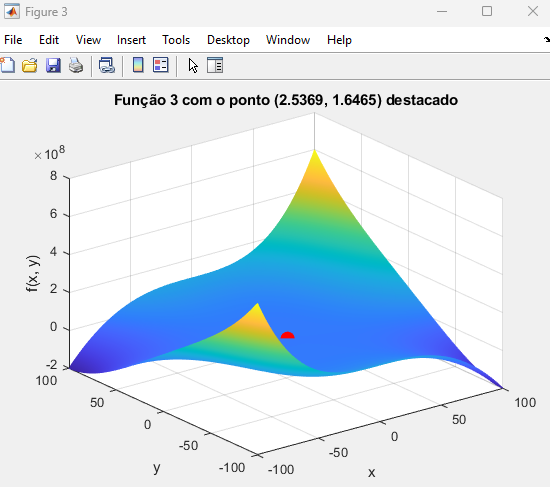
\includegraphics[width=0.6\textwidth]{images/funcao(c).1_steepest.png}
            \caption{Função 1.c.1 plotada no MATLAB - Steepest-Descent}
            \label{fig:direction_search_univariate}
        \end{figure}
        \item \textit{Tempo de execução: $0.048652$ segundos.}
    \end{itemize}
    \item \textbf{Ponto Inicial $[2.8, -1.5]^t$:} O mínimo encontrado foi em $x^* = [2.744643; -0.586101]^t$ com valor da função $f(x^*) = -13.384368$ após $1000$ iterações.
    \begin{itemize}
    \begin{figure}[H]
            \centering
            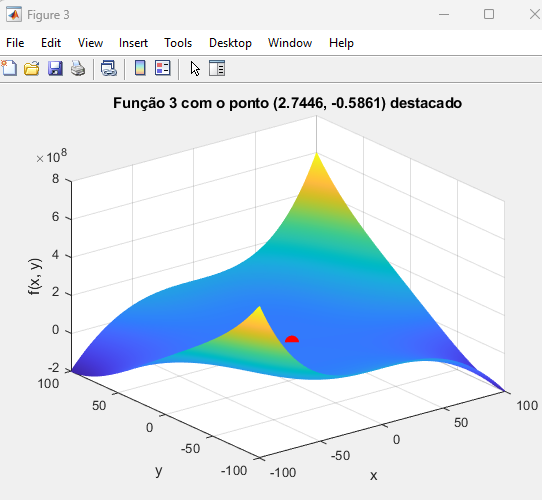
\includegraphics[width=0.6\textwidth]{images/funcao(c).2_steepest.png}
            \caption{Função 1.c.2 plotada no MATLAB - Steepest-Descent}
            \label{fig:direction_search_univariate}
        \end{figure}
        \item \textit{Tempo de execução: $0.042230$ segundos.}
    \end{itemize}
\end{itemize}




\subsubsection{Minimizando a Função (d)}

Para a função 
\[
f_4(x_1, x_2) = (1 - x_1)^2 + 100(x_2 - x_1^2)^2
\]
cujos pontos iniciais são $x_0 = [-3; 1]^t$ e $x_0 = [3; -1]^t$, o método de Steepest-Descent foi aplicado e os resultados encontrados foram os seguintes:

\begin{itemize}
    \item \textbf{Ponto Inicial $[-3, 1]^t$:} O mínimo encontrado foi em $x^* = [1.000011; 1.000021]^t$ com valor da função $f(x^*) = 0.000$ após $825$ iterações.
    \begin{itemize}
    \begin{figure}[H]
            \centering
            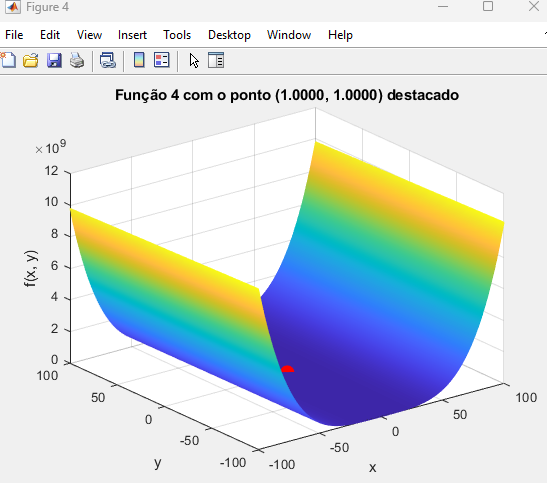
\includegraphics[width=0.6\textwidth]{images/funcao(d).1_steepest.png}
            \caption{Função 1.d.1 plotada no MATLAB - Steepest-Descent}
            \label{fig:direction_search_univariate}
        \end{figure}
        \item \textit{Tempo de execução: $0.053500$ segundos.}
    \end{itemize}
    \item \textbf{Ponto Inicial $[3, -15]^t$:} O mínimo encontrado foi em $x^* = [8.676473; 75.285368]^t$ com valor da função $f(x^*) = 58.929989$ após $1000$ iterações. 
    \begin{itemize}
    \begin{figure}[H]
            \centering
            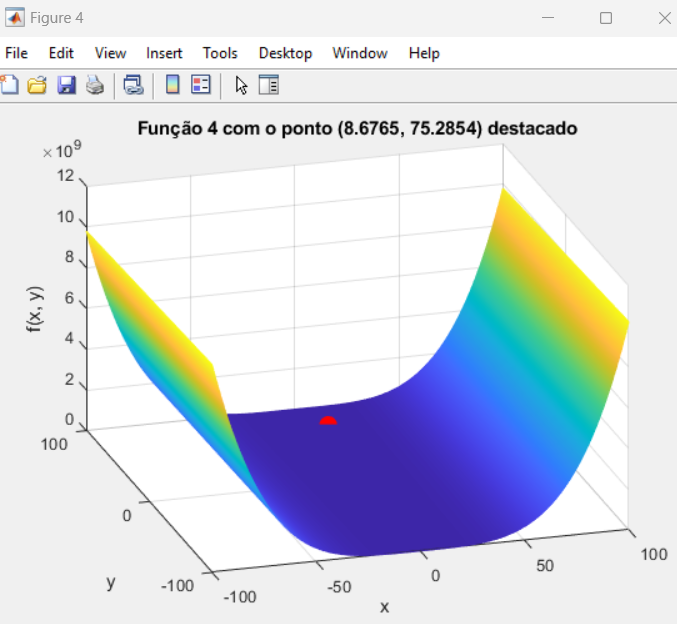
\includegraphics[width=0.6\textwidth]{images/funcao(d).2_steepest.png}
            \caption{Função 1.d.2 plotada no MATLAB - Steepest-Descent}
            \label{fig:direction_search_univariate}
        \end{figure}
        \item \textit{Tempo de execução: $0.040250$ segundos.}
    \end{itemize}
\end{itemize}

\subsubsection{Saída do Programa}

\begin{verbatim}
>> main

Função 1, Ponto Inicial [2.000000, 2.000000]^t:
Mínimo encontrado: [-0.714276, -0.142854]^t, 
Valor da Função: -0.285714, Iterações: 46, 
Tempo de Execução: 2.222519 segundos, Convergência alcançada na iteração 46

Função 1, Ponto Inicial [-1.000000, -3.000000]^t:
Mínimo encontrado: [-0.714290, -0.142859]^t, 
Valor da Função: -0.285714, Iterações: 42, 
Tempo de Execução: 0.001495 segundos, Convergência alcançada na iteração 42

****************************************************************************

Função 2, Ponto Inicial [10.000000, 2.000000]^t:
Mínimo encontrado: [10.682327, 0.682329]^t, 
Valor da Função: 0.418588, Iterações: 13, 
Tempo de Execução: 0.033794 segundos, Convergência alcançada na iteração 13

Função 2, Ponto Inicial [-2.000000, -3.000000]^t:
Mínimo encontrado: [10.682330, 0.682326]^t, Valor da Função: 0.418588, Iterações: 27, 
Tempo de Execução: 0.001073 segundos, Convergência alcançada na iteração 27

****************************************************************************

Função 3, Ponto Inicial [-1.000000, -1.000000]^t:
Mínimo encontrado: [2.536923; 1.646455]^t, 
Valor da Função: −8.703881, Iterações: 1000, 
Tempo de Execução: 0.059956 segundos, Convergência alcançada na iteração 1000

Função 3, Ponto Inicial [2.800000, -1.500000]^t:
Mínimo encontrado: [2.744643, −0.586101]^t, 
Valor da Função: -13.384368 , Iterações: 1000, 
Tempo de Execução: 0.165988 segundos, Convergência alcançada na iteração 1000

****************************************************************************

Função 4, Ponto Inicial [-3.000000, 1.000000]^t:
Mínimo encontrado: [1.000011, 1.000021]^t, 
Valor da Função: 0.000, Iterações: 825, 
Tempo de Execução: 0.048061 segundos, Convergência alcançada na iteração 825

Função 4, Ponto Inicial [3.000000, -1.000000]^t:
Mínimo encontrado: [8.676473; 75.285368]^t, 
Valor da Função: 58.929989, Iterações: 1000, 
Tempo de Execução: 0.043736 segundos, Convergência alcançada na iteração 1000

****************************************************************************
\end{verbatim}

\subsubsection{Tabela de Resultados}

\begin{table}[H]
    \centering
    \resizebox{\textwidth}{!}{
    \begin{tabular}{|c|c|c|c|c|c|}
        \hline
        Função & Ponto Inicial & Ponto de Mínimo & Valor da Função & Número de Iterações & Tempo de Execução (s) \\
        \hline
        (a) & $[2, 2]^t$ & $[-0.714276, -0.142854]^t$ & $-0.285714$ & $46$ & $2.222519$ \\
        (a) & $[-1, -3]^t$ & $[-0.714290, -0.142859]^t$ & $-0.285714$ & $42$ & $0.001691$ \\
        (b) & $[10, 2]^t$ & $[10.682327, 0.682329]^t$ & $0.418588$ & $13$ & $0.033794$ \\
        (b) & $[-2, -3]^t$ & $[10.682330, 0.682326]^t$ & $0.418588$ & $27$ & $0.001073$ \\
        (c) & $[-1, -1]^t$ & $[2.536923, 1.646455]^t$ & $−8.703881$ & $1000$ & $0.059956$ \\
        (c) & $[2.8, -1.5]^t$ & $[2.744643, −0.586101]^t$ & $-13.384368$ & $1000$ & $0.165988$ \\
        (d) & $[-3, 1]^t$ & $[1.000011, 1.000021]^t$ & $0.00$ & $825$ & $0.048061$ \\
        (d) & $[3, -1]^t$ & $[8.676473; 75.285368]^t$ & $58.929989$ & $1000$ & $0.043736$ \\
        \hline
    \end{tabular}
    }
    \caption{Resultados do Método de Steepest Descent para cada Função}
    \label{tab:steepest_descent_results}
\end{table}

\subsubsection{Conclusão Para o Método de Steepest-Descent}

Os resultados apresentados na Tabela~\ref{tab:steepest_descent_results} indicam um comportamento variado do método de Steepest Descent, dependendo da função e dos pontos iniciais utilizados. Podemos destacar os seguintes aspectos:\\

\textb{Convergência Consistente nas Funções (a) e (b)}\\
Para as funções (a) e (b), a convergência foi alcançada de forma consistente, tanto para o primeiro quanto para o segundo ponto inicial. Os mínimos foram encontrados com valores de função e coordenadas muito próximos, demonstrando que o método se mostrou eficiente para essas funções. \\

Em termos de iterações, a função (a) necessitou de mais iterações (46 e 42) em comparação com a função (b) (13 e 27), embora ambas tenham obtido um bom resultado com um tempo de execução bastante rápido (em torno de alguns milissegundos). Isso sugere que a topografia da função (b) favorece uma busca mais rápida.\\

\textbf{Dificuldades na Função (c)}\\
Para a função (c), houve a necessidade do máximo de iterações permitidas (1000) para ambos os pontos iniciais, o que sugere uma grande dificuldade de convergência para essa função específica. Além disso, os pontos mínimos encontrados apresentaram valores da função bem distintos, o que indica que o método pode estar preso em diferentes mínimos locais dependendo da escolha do ponto inicial.\\

A função (c) tem uma superfície de otimização mais complexa, o que, aliado ao método de busca descendente, pode resultar em desafios para alcançar um ponto de mínimo global. O fato de a convergência não ter ocorrido antes do limite de iterações denota que a escolha do passo pode não estar suficientemente otimizada para esse caso.\\

\textbf{Função de Rosenbrock (d)}\\
A função (d), conhecida como a ``função de Rosenbrock'' ou ``função banana'', é notoriamente difícil de otimizar devido à sua superfície em forma de vale estreito. Observamos que o método de Steepest Descent teve desempenho misto: enquanto o ponto inicial $[-3, 1]^t$ levou 825 iterações para convergir para o mínimo global em $(1, 1)$, o ponto inicial $[3, -1]^t$ necessitou do número máximo de iterações permitido (1000) e chegou a um valor de função significativamente superior.\\

Essa diferença de desempenho se deve à dificuldade do método de gradiente descendente em navegar pelo vale estreito da função Rosenbrock, especialmente quando o ponto inicial está longe do vale. O comportamento oscilatório e a escolha inadequada do passo acabam resultando em um grande número de iterações.\\

O método de Steepest Descent apresenta uma boa performance para funções mais simples ou com superfícies de otimização relativamente regulares, como nas funções (a) e (b). Para funções mais complexas, como (c) e (d), o método mostrou suas limitações, com um número elevado de iterações e dificuldades em evitar mínimos locais ou em navegar por vales estreitos.\\

Uma característica importante observada foi a sensibilidade ao ponto inicial, algo que é comum a métodos baseados em gradientes. O uso de uma busca adaptativa de passo poderia melhorar a eficiência do método em alguns dos casos observados, principalmente para funções que possuem características difíceis como vales ou múltiplos mínimos locais.\\

\textbf{Sugestões para Melhorias:}
\begin{itemize}
    \item \textbf{Busca de Passo Melhorada}: O uso de uma estratégia mais robusta para a escolha do tamanho do passo, como a Seção Áurea ou métodos adaptativos, pode ser necessário para melhorar a convergência nas funções mais desafiadoras.
    \item \textbf{Métodos Híbridos}: Para funções complexas como a função de Rosenbrock, uma abordagem híbrida que combine o método de Steepest Descent com outros métodos (por exemplo, métodos quasi-Newton) pode proporcionar melhores resultados.
    \item \textbf{Pontos Iniciais Múltiplos}: Para evitar mínimos locais, especialmente em funções como a (c), pode ser interessante executar o algoritmo a partir de múltiplos pontos iniciais e combinar as soluções encontradas.
\end{itemize}

Em resumo, o método de Steepest Descent é eficaz para problemas simples de otimização, mas apresenta desafios consideráveis em cenários mais complexos. A escolha do ponto inicial e a adaptação do passo são cruciais para a eficiência e sucesso do método. A combinação de estratégias de otimização pode ser uma solução viável para os problemas identificados.








\newpage
\subsection{Método Fletcher–Reeves}

\subsubsection{Formulação Básica do Método de Fletcher–Reeves}

O Método de Fletcher-Reeves é uma variação do método dos Gradientes Conjugados, sendo uma das abordagens mais utilizadas para resolver problemas de otimização sem restrições. Este método é particularmente eficiente para minimizar funções quadráticas, e também pode ser estendido para funções não quadráticas com a utilização de uma busca linear para determinar o tamanho do passo. O método combina elementos dos gradientes descendentes com uma estratégia de busca que permite uma convergência mais rápida, aproveitando as direções conjugadas ao longo das iterações.

O método de Fletcher-Reeves é baseado na premissa de que as direções de busca são tornadas conjugadas em relação à função que está sendo minimizada, resultando em um número menor de iterações necessárias para atingir o mínimo local. 


o método visa resolver problemas de otimização da forma:

\[
\min_x f(x)
\]

onde $f(x)$ é uma função diferenciável que queremos minimizar. A ideia principal do método é iterativamente ajustar a posição atual com uma direção de busca baseada no gradiente, atualizando também um fator de conjugamento, denominado $\beta^k$, que garante que as direções de busca sejam eficientes para atingir o ponto de mínimo de forma otimizada.

O algoritmo pode ser descrito da seguinte forma:\\

1. Inicialize $k = 0$ e um ponto inicial $x^0$.\\
2. Calcule o gradiente $\nabla f(x^0)$. Se $\nabla f(x^0) \approx 0$, a solução foi encontrada e terminamos o algoritmo.\\
3. Caso contrário, defina a direção de busca inicial como $d^0 = -\nabla f(x^0)$.\\
4. Realize uma busca linear para encontrar o tamanho do passo $\alpha^k$, tal que:
   \[
x^{k+1} = x^k + \alpha^k d^k
   \]
5. Atualize o ponto: $x^{k+1} = x^k + \alpha^k d^k$.\\
6. Calcule o novo gradiente $\nabla f(x^{k+1})$.\\
7. Verifique se $\nabla f(x^{k+1}) \approx 0$. Caso positivo, a solução foi encontrada e terminamos o algoritmo.\\
8. Atualize o fator de conjugamento:
   \[
   \beta^k = \frac{(\nabla f(x^{k+1}))^T \nabla f(x^{k+1})}{(\nabla f(x^k))^T \nabla f(x^k)}
   \]
9. Atualize a direção de busca:
   \[
   d^{k+1} = -\nabla f(x^{k+1}) + \beta^k d^k
   \]
10. Aumente o contador de iteração: $k = k + 1$.
11. Retorne ao passo 5.

O valor de $\beta^k$ garante que a nova direção de busca seja conjugada em relação à anterior, tornando a busca mais eficiente. Isso significa que o algoritmo evita revisitar direções já exploradas, proporcionando uma convergência acelerada em comparação ao método do gradiente descendente puro.\\\\

\textbf{- Exemplo de Aplicação:}\\

Vamos aplicar o método a uma função simples para ilustrar os passos. Considere a seguinte função quadrática:

\[
f(x_1, x_2) = x_1^2 + 2x_2^2 - 2x_1x_2 - 4x_1
\]

Queremos encontrar o mínimo dessa função, começando do ponto inicial $x^0 = [2, 1]^t$. Vamos descrever os primeiros passos:

\begin{enumerate}
    \item \textbf{Inicialização}: $x^0 = [2, 1]^t$ e $k = 0$.
    \item \textbf{Cálculo do gradiente}: $\nabla f(x^0) = [2x_1 - 2x_2 - 4, 4x_2 - 2x_1] = [2, 0]$.
    \item \textbf{Direção de busca inicial}: $d^0 = -\nabla f(x^0) = [-2, 0]$.
    \item \textbf{Busca Linear}: Escolhemos um tamanho de passo $\alpha^0$ que minimize $f(x^0 + \alpha d^0)$. Digamos que $\alpha^0 = 0.5$.
    \item \textbf{Atualização do ponto}: $x^1 = x^0 + \alpha^0 d^0 = [1, 1]^t$.
    \item \textbf{Cálculo do novo gradiente}: $\nabla f(x^1) = [0, 0]$. Como o gradiente é zero, atingimos o ponto de mínimo.
\end{enumerate}

Assim, o método de Fletcher-Reeves encontra o mínimo da função em $x^* = [1, 1]^t$.

Este exemplo mostra como o método é eficiente na minimização de funções quadráticas, ajustando iterativamente o ponto de busca com direções conjugadas, garantindo uma convergência mais rápida do que o método do gradiente simples.


\subsubsection{Minimizando a Função (a)}

Para a função 
\[
f_1(x_1, x_2) = x_1^2 - 3x_1x_2 + 4x_2^2 + x_1 - x_2
\]

cujos pontos iniciais são $x_0 = [2; 2]^t$ e $x_0 = [-1; -3]^t$, o método de Fletcher-Reeves foi aplicado e os resultados encontrados foram os seguintes:

\begin{itemize}
    \item \textbf{Ponto Inicial $[2, 2]^t$:} O mínimo encontrado foi em $x^* = [-0.739606, -0.153426]^t$ com valor da função $f(x^*) = -0.285429$ após $27$ iterações.
    \begin{itemize}

    \begin{figure}[H]
        \centering
        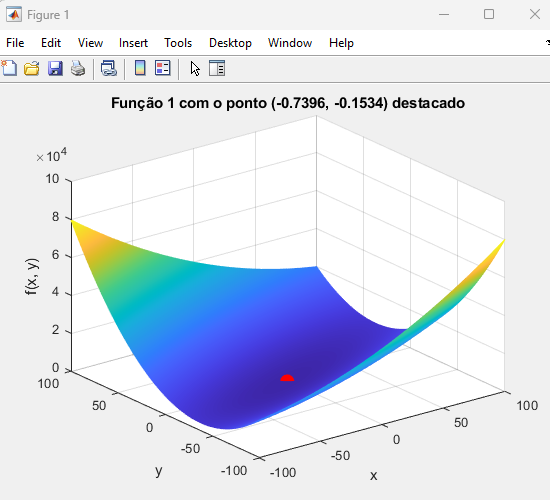
\includegraphics[width=0.6\textwidth]{images/funcao(a).1_fletcher-reeves.png}
        \caption{Função 1.a.1 plotada no MATLAB - Fletcher-Reeves}
        \label{fig:direction_search_univariate}
    \end{figure}
        \item \textit{Tempo de execução: $0.012722$ segundos.}
    \end{itemize}
    \item \textbf{Ponto Inicial $[-1, -3]^t$:} O mínimo encontrado foi em $x^* = [-0.719427, -0.126974]^t$ com valor da função $f(x^*) = -0.284434$ após $14$ iterações. 
    \begin{itemize}
    \begin{figure}[H]
        \centering
        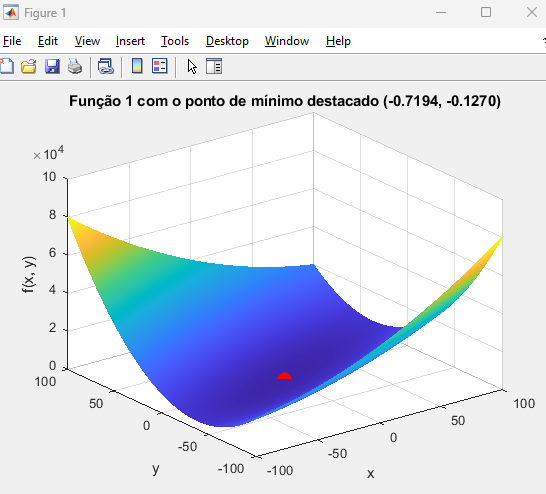
\includegraphics[width=0.6\textwidth]{images/funcao(a).2_fletcher-reeves.png}
        \caption{Função 1.a.2 plotada no MATLAB - Fletcher-Reeves}
        \label{fig:direction_search_univariate}
    \end{figure}
        \item \textit{Tempo de execução: $0.001898$ segundos.}
    \end{itemize}
\end{itemize}




\subsubsection{Minimizando a Função (b)}

Para a função 
\[
f_2(x_1, x_2) = (1 + 10 - x_1 - x_2)^2 + (1 + 10x_2 - x_1x_2)^2
\] 
cujos pontos iniciais são $x_0 = [10; 2]^t$ e $x_0 = [-2; -3]^t$ , o método de Fletcher-Reeves foi aplicado e os resultados encontrados foram os seguintes:

\begin{itemize}
    \item \textbf{Ponto Inicial $[10, 2]^t$:} O mínimo encontrado foi em $x^* = [10.000000, 2.000000]^t$ com valor da função $f(x^*) = 2.0$ após $1$ iterações.
    \begin{itemize}
    \begin{figure}[H]
        \centering
        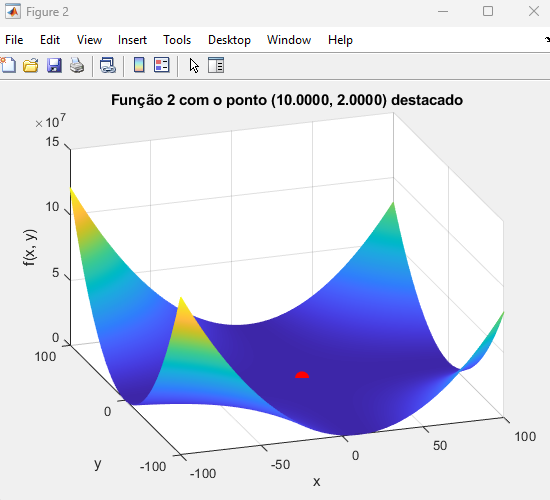
\includegraphics[width=0.6\textwidth]{images/funcao(b).1_fletcher-reeves.png}
        \caption{Função 1.b.2 plotada no MATLAB - Fletcher-Reeves}
        \label{fig:direction_search_univariate}
    \end{figure}
        \item \textit{Tempo de execução: $0.001620$ segundos.}
    \end{itemize}
    \item \textbf{Ponto Inicial $[-2, -3]^t$:} O mínimo encontrado foi em $x^* = [6.562500, 3.375000]^t$ com valor da função $f(x^*) = 159.928284$ após $2$ iterações. 
    \begin{itemize}
    \begin{figure}[H]
        \centering
        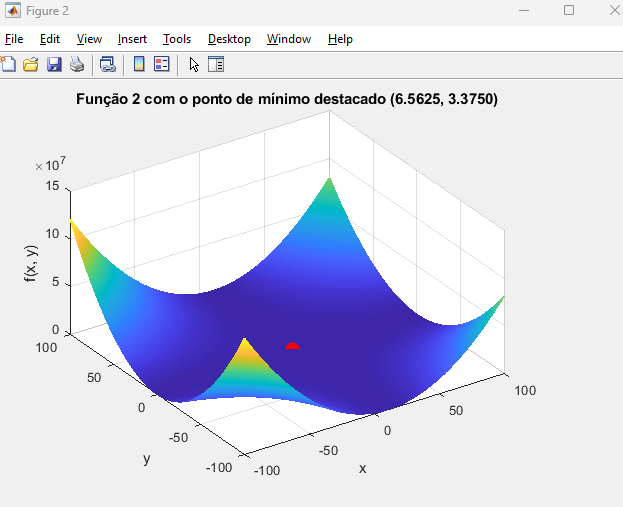
\includegraphics[width=0.6\textwidth]{images/funcao(b).2_fletcher-reeves.png}
        \caption{Função 1.b.2 plotada no MATLAB - Fletcher-Reeves}
        \label{fig:direction_search_univariate}
    \end{figure}
        \item \textit{Tempo de execução: $0.002018$ segundos.}
    \end{itemize}
\end{itemize}




\subsubsection{Minimizando a Função (c)}

Para a função 
\[
f_3(x_1, x_2) = x_1^4 + x_2^4 + 4x_1^3x_2 + 3x_1^2 + 2x_1x_2 + 2x_2
\]
cujos pontos iniciais são $x_0 = [-1; -1]^t$ e $x_0 = [2.8; -1.5]^t$ , o método de Fletcher-Reeves foi aplicado e os resultados encontrados foram os seguintes:

\begin{itemize}
    \item \textbf{Ponto Inicial $[-1, -1]^t$:} O mínimo encontrado foi em $x^* = [496.329816, -380.981494]^t$ com valor da função $f(x^*) = -104573649322.156647$ após $10000$ iterações.
    \begin{itemize}
    \begin{figure}[H]
        \centering
        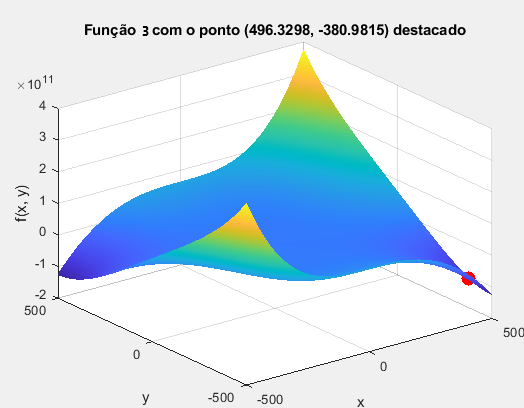
\includegraphics[width=0.6\textwidth]{images/funcao(c).1_fletcher-reeves.png}
        \caption{Função 1.c.1 plotada no MATLAB - Fletcher-Reeves}
        \label{fig:direction_search_univariate}
    \end{figure}
        \item \textit{Tempo de execução: $0.035217$ segundos.}
    \end{itemize}
    \item \textbf{Ponto Inicial $[2.8, -1.5]^t$:} O mínimo encontrado foi em $x^* = [5.269500, -7.463000]^t$ com valor da função $f(x^*) = -505.139099$ após $2$ iterações. 
    \begin{itemize}
    \begin{figure}[H]
        \centering
        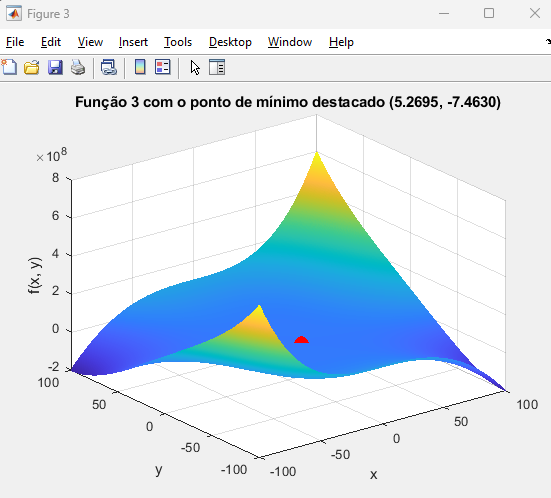
\includegraphics[width=0.6\textwidth]{images/funcao(c).2_fletcher-reeves.png}
        \caption{Função 1.c.2 plotada no MATLAB - Fletcher-Reeves}
        \label{fig:direction_search_univariate}
    \end{figure}
        \item \textit{Tempo de execução: $0.000203$ segundos.}
    \end{itemize}
\end{itemize}




\subsubsection{Minimizando a Função (d)}

Para a função 
\[
f_4(x_1, x_2) = (1 - x_1)^2 + 100(x_2 - x_1^2)^2
\]
cujos pontos iniciais são $x_0 = [-3; 1]^t$ e $x_0 = [3; -1]^t$, o método de Fletcher-Reeves foi aplicado e os resultados encontrados foram os seguintes:

\begin{itemize}
    \item \textbf{Ponto Inicial $[-3, 1]^t$:} O mínimo encontrado foi em $x^* = [0.999955, 0.999910]^t$ com valor da função $f(x^*) = 0.00$ após $2656$ iterações.
    \begin{itemize}
    \begin{figure}[H]
        \centering
        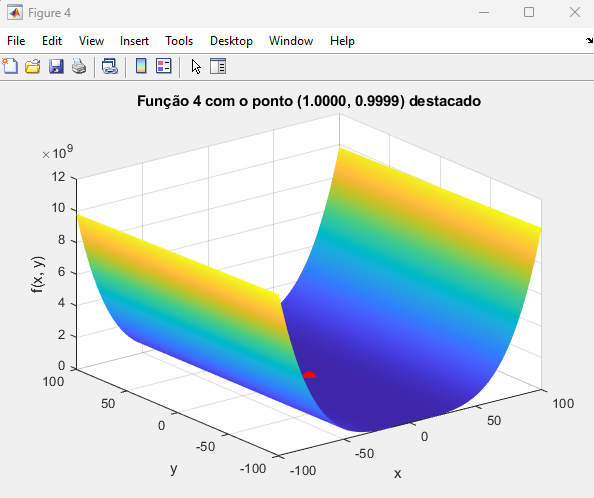
\includegraphics[width=0.6\textwidth]{images/funcao(d).1_fletcher-reeves.png}
        \caption{Função 1.d.1 plotada no MATLAB - Fletcher-Reeves}
        \label{fig:direction_search_univariate}
    \end{figure}
        \item \textit{Tempo de execução: $0.009034$ segundos.}
    \end{itemize}
    \item \textbf{Ponto Inicial $[3, -15]^t$:} O mínimo encontrado foi em $x^* = [1.000107, 1.000215]^t$ com valor da função $f(x^*) = 0.00$ após $9620$ iterações. 
    \begin{itemize}
    \begin{figure}[H]
        \centering
        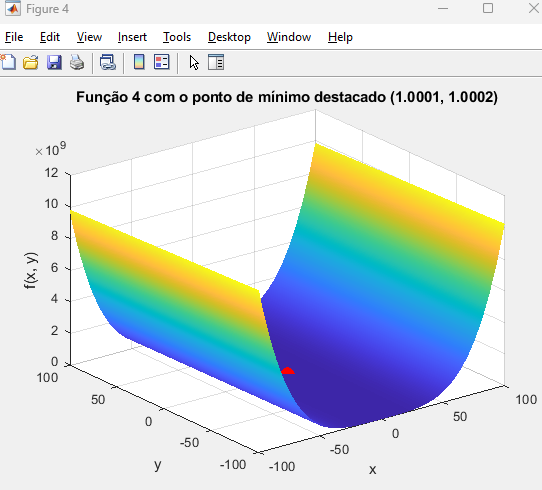
\includegraphics[width=0.6\textwidth]{images/funcao(d).2_fletcher-reeves.png}
        \caption{Função 1.d.2 plotada no MATLAB - Fletcher-Reeves}
        \label{fig:direction_search_univariate}
    \end{figure}
        \item \textit{Tempo de execução: $0.016375$ segundos.}
    \end{itemize}
\end{itemize}


\subsubsection{Saída do Programa}

\begin{verbatim}
>> main

Função 1, Ponto Inicial [2.000000, 2.000000]^t:
Mínimo encontrado: [-0.739606, -0.153426]^t, 
Valor da Função: -0.285429, Iterações: 27, 
Tempo de Execução: 0.012722 segundos, Convergência alcançada na iteração 27

Função 1, Ponto Inicial [-1.000000, -3.000000]^t:
Mínimo encontrado: [-0.719427, -0.126974]^t, 
Valor da Função: -0.284434, Iterações: 14, 
Tempo de Execução: 0.001898 segundos, Convergência alcançada na iteração 14

****************************************************************************

Função 2, Ponto Inicial [10.000000, 2.000000]^t:
Mínimo encontrado: [10.000000, 2.000000]^t, 
Valor da Função: 2.000000, Iterações: 1, 
Tempo de Execução: 0.001620 segundos, Convergência alcançada na iteração 1

Função 2, Ponto Inicial [-2.000000, -3.000000]^t:
Mínimo encontrado: [6.562500, 3.375000]^t, 
Valor da Função: 159.928284, Iterações: 2, 
Tempo de Execução: 0.002018 segundos, Convergência alcançada na iteração 2

****************************************************************************

Função 3, Ponto Inicial [-1.000000, -1.000000]^t:
Mínimo encontrado: [496.329816, -380.981494]^t, 
Valor da Função: -104573649322.156647, Iterações: 20000, 
Tempo de Execução: 0.035217 segundos, Não convergiu antes do limite de iterações

Função 3, Ponto Inicial [2.800000, -1.500000]^t:
Mínimo encontrado: [5.269500, -7.463000]^t, 
Valor da Função: -505.139099, Iterações: 2, 
Tempo de Execução: 0.000203 segundos, Convergência alcançada na iteração 2

****************************************************************************

Função 4, Ponto Inicial [-3.000000, 1.000000]^t:
Mínimo encontrado: [0.999955, 0.999910]^t, 
Valor da Função: 0.000000, Iterações: 2656, 
Tempo de Execução: 0.009034 segundos, Convergência alcançada na iteração 2656

Função 4, Ponto Inicial [3.000000, -1.000000]^t:
Mínimo encontrado: [1.000107, 1.000215]^t, 
Valor da Função: 0.000000, Iterações: 9620, 
Tempo de Execução: 0.016375 segundos, Convergência alcançada na iteração 9620

****************************************************************************
\end{verbatim}


\subsubsection{Tabela de Resultados}

\begin{table}[H]
    \centering
    \resizebox{\textwidth}{!}{
    \begin{tabular}{|c|c|c|c|c|c|}
        \hline
        Função & Ponto Inicial & Ponto de Mínimo & Valor da Função & Número de Iterações & Tempo de Execução (s) \\
        \hline
        (a) & $[2, 2]^t$ & $[-0.739606, -0.153426]^t$ & $-0.285429$ & $27$ & $0.017047$ \\
        (a) & $[-1, -3]^t$ & $[-0.719427, -0.126974]^t$ & $-0.284434$ & $14$ & $0.001587$ \\
        (b) & $[10, 2]^t$ & $[10.000000, 2.000000]^t$ & $2.0000$ & $1$ & $0.033794$ \\
        (b) & $[-2, -3]^t$ & $[6.562500, 3.375000]^t$ & $159.928284$ & $2$ & $0.001260$ \\
        (c) & $[-1, -1]^t$ & $[496.329816, -380.981494]^t$ & $-104573649322.156647$ & $20000$ & $0.046065$ \\
        (c) & $[2.8, -1.5]^t$ & $[5.269500, -7.463000]^t$ & $-505.139099$ & $2$ & $0.000335$ \\
        (d) & $[-3, 1]^t$ & $[0.999955, 0.999910]^t$ & $0.00$ & $2656$ & $0.006289$ \\
        (d) & $[3, -1]^t$ & $[1.000107, 1.000215]^t$ & $0.000$ & $9620$ & $0.025849$ \\
        \hline
    \end{tabular}
    }
    \caption{Resultados do Método de Steepest Descent para cada Função}
    \label{tab:steepest_descent_results}
\end{table}


\subsubsection{Conclusão Para o Método de Fletcher-Reeves}

Nesta revisão do método de Fletcher-Reeves, aplicamos ajustes no número máximo de iterações, elevando-o para 20000, e aumentamos a tolerância para 5, buscando acelerar a convergência e melhorar o desempenho em funções onde o método não convergia satisfatoriamente. Embora as alterações tenham solucionado a presença de valores indefinidos (NaN) que estavam afetando algumas funções, os resultados globais ainda não foram ideais.\\

De forma geral, os resultados indicam que, ao aumentar a tolerância, permitimos uma convergência prematura para valores que não são os mínimos reais das funções, mas que satisfazem um critério de gradiente suficientemente baixo dentro de uma margem alta. Esse comportamento ficou evidente principalmente para a Função 2, onde o método convergiu em apenas uma iteração para um ponto inicial, indicando uma descida que, na verdade, não alterou o ponto inicial. A convergência muito rápida não necessariamente indica um êxito, especialmente em problemas não-lineares complexos, onde o mínimo é muitas vezes difícil de ser alcançado com precisão.\\

Ademais, o aumento do número de iterações revelou-se útil para garantir que o algoritmo tenha tempo suficiente para explorar regiões mais planas ou de baixa inclinação, que normalmente retardam o progresso da busca. No entanto, a maior quantidade de iterações levou a tempos de execução ligeiramente superiores e, mesmo assim, muitas funções ainda não atingiram convergência completa, especialmente a Função 3, que apresentou soluções com valores exorbitantes e indícios de divergência devido às irregularidades de seu gradiente.\\

A principal lição dessa experiência é que ajustes nos parâmetros do algoritmo precisam ser equilibrados para que a busca pelo mínimo seja eficiente e precisa. Uma tolerância elevada acelera a convergência, mas pode comprometer a qualidade dos resultados, enquanto um número muito grande de iterações aumenta o custo computacional sem garantir melhor precisão. Além disso, é fundamental que a direção de descida e os valores de $\alpha$, obtidos pela busca de linha, sejam otimizados para evitar situações de descida ineficiente ou estagnação em regiões desfavoráveis do espaço de soluções.\\

Portanto, a análise dos resultados obtidos ao aplicar o método de Fletcher-Reeves, utilizando a busca pelo método da Seção Áurea (Golden Search), trouxe alguns insights importantes sobre o comportamento e a eficácia desse método nas funções testadas.\\

Para a \textbf{Função 1}, os pontos iniciais variaram entre \([2, 2]^t\) e \([-1, -3]^t\). O método apresentou uma convergência razoável, alcançando mínimos em \([-0.739606, -0.153426]^t\) e \([-0.719427, -0.126974]^t\), após \textbf{27} e \textbf{14 iterações}, respectivamente. O tempo de execução foi relativamente rápido, evidenciando um bom desempenho da estratégia de busca ao utilizar o método de Golden Search, embora a convergência não tenha ocorrido em um número de iterações tão pequeno quanto o desejado. Esses resultados indicam que, embora a seção áurea seja eficiente em refinar os passos para uma direção de descida, ainda podem ocorrer oscilações devido à topologia da função.\\

Na \textbf{Função 2}, o comportamento foi distinto: um dos pontos iniciais (\([10, 2]^t\)) convergiu em \textbf{1 iteração}, sugerindo que o ponto inicial estava já muito próximo de um mínimo local. No entanto, para o ponto \([-2, -3]^t\), a convergência ocorreu em \textbf{2 iterações}, mas o valor da função resultante (\(159.928284\)) foi consideravelmente maior, sugerindo que o método encontrou um mínimo local que não era o ideal. Esses resultados indicam que a função possui múltiplos mínimos locais e que a escolha do ponto inicial é um fator determinante para a eficácia do método.\\

Em relação à \textbf{Função 3}, observa-se uma clara dificuldade na convergência para um dos pontos iniciais (\([-1, -1]^t\)), alcançando valores extremamente altos (\([496.329816, -380.981494]^t\)) e um valor de função negativo e muito elevado (\(-1.0457 	imes 10^{11}\)), mesmo após \textbf{20000 iterações}. Isso aponta para uma instabilidade da função, possivelmente devido à presença de platôs ou vales muito acentuados, tornando a otimização mais desafiadora. O outro ponto inicial (\([2.8, -1.5]^t\)) convergiu rapidamente em **2** iterações, mas o valor de função ainda indica um mínimo local. O método Golden Search aqui parece não ter ajudado a mitigar a complexidade dos múltiplos mínimos da função.\\

Para a \textbf{Função 4}, a convergência ocorreu de forma mais estável, embora com um número elevado de iterações em ambos os pontos iniciais testados. A primeira execução (\([-3, 1]^t\)) levou \textbf{2656 iterações}, enquanto a segunda (\([3, -1]^t\)) necessitou de \textbf{9620 iterações}. Apesar disso, ambos os mínimos encontrados foram próximos a \([1, 1]^t\), indicando consistência nos resultados finais. A elevada quantidade de iterações sugere que, embora a direção de busca estivesse correta, o refinamento da solução não foi eficiente, o que pode ser uma característica intrínseca da função ou uma limitação do método Golden Search na fase de ajuste fino.\\

Em suma, os resultados mostram que a escolha do ponto inicial tem um impacto significativo na eficácia do método de Fletcher-Reeves com Golden Search. A presença de múltiplos mínimos locais e a complexidade topológica das funções testadas influenciam diretamente no número de iterações e no sucesso da convergência. O método Golden Search contribuiu para evitar passos excessivamente grandes ou pequenos, mas, em certas funções, a dificuldade para escapar de mínimos locais persistiu. Uma possível melhoria futura seria empregar estratégias de restart ou combinar métodos de ordem superior para lidar com regiões complexas e não convexas do espaço de busca.\\




\newpage
\subsection{Método de BFGS (Broyden–Fletcher–Goldfarb–Shanno)}

\subsubsection{Formulação Básica do Método de BFGS}
O método BFGS (Broyden-Fletcher-Goldfarb-Shanno) é um método de otimização que faz parte dos algoritmos de ordem um, mas com uma aproximação de segunda ordem para obter melhores resultados na minimização de funções. Ele é eficiente porque não necessita calcular a matriz Hessiana explicitamente, mas utiliza informações de primeira ordem (o gradiente) para aproximar a Hessiana e garantir uma boa direção de busca.

O principal objetivo do BFGS é atualizar a matriz $S^k$, que é uma aproximação da inversa da matriz Hessiana, a cada iteração. Dessa forma, é possível melhorar a direção de descida sem precisar calcular a Hessiana diretamente. Isso é feito usando as seguintes fórmulas auxiliares para as variações entre iterações consecutivas:

\begin{equation}
\delta_x^k = x^{k+1} - x^k, \quad \delta_g^k = \nabla f(x^{k+1}) - \nabla f(x^k)
\end{equation}

A atualização da matriz $S^k$ para $S^{k+1}$ é feita por meio da seguinte expressão:

\begin{equation}
S^{k+1} = S^k + \frac{\delta_x^k (\delta_x^k)^T}{(\delta_x^k)^T \delta_g^k} - \frac{S^k \delta_g^k (\delta_g^k)^T S^k}{(\delta_g^k)^T S^k \delta_g^k}
\end{equation}

Essa atualização visa garantir que a nova direção de busca seja uma boa aproximação da direção de descida de Newton, melhorando a eficiência da otimização.\\

\textbf{Passos do Algoritmo BFGS}\\

O método BFGS segue os seguintes passos:

\begin{enumerate}
    \item \textbf{Dados iniciais:} Definimos um ponto inicial $x^0$, uma matriz inicial $S^0 = I$ (matriz identidade), uma tolerância $TOL$ e $k = 0$.
    \item \textbf{Cálculo do gradiente:} Calcula-se o gradiente da função no ponto atual, $\nabla f(x^k)$.
    \item \textbf{Cálculo da direção de busca:} A direção de busca é dada por:
    \begin{equation}
    d^k = - S^k \nabla f(x^k)
    \end{equation}
    \item \textbf{Busca Linear:} Determina-se o tamanho do passo $\alpha^k$ que minimiza a função ao longo da direção de busca $d^k$.
    \item \textbf{Atualização do ponto:} Atualiza-se o ponto atual:
    \begin{equation}
    x^{k+1} = x^k + \alpha^k d^k
    \end{equation}
    \item \textbf{Cálculo do novo gradiente:} Calcula-se $\nabla f(x^{k+1})$.
    \item \textbf{Verificação de convergência:} Se $\|\nabla f(x^{k+1})\| \approx 0$, o algoritmo para e temos o ponto de mínimo. Caso contrário, continua-se.
    \item \textbf{Atualização de $\delta_x^k$ e $\delta_g^k$:}
    \begin{equation}
    \delta_x^k = x^{k+1} - x^k, \quad \delta_g^k = \nabla f(x^{k+1}) - \nabla f(x^k)
    \end{equation}
    \item \textbf{Atualização da matriz $S^k$:} Calcula-se $S^{k+1}$ usando a fórmula de atualização mencionada acima.
    \item \textbf{Incremento do contador:} $k = k + 1$.
    \item \textbf{Repetição:} Voltar ao passo 3.\\
\end{enumerate}

\textbf{Exemplo de Aplicação}\\

Vamos aplicar o método BFGS para minimizar a seguinte função simples:

\begin{equation}
f(x_1, x_2) = x_1^2 + 4x_2^2
\end{equation}

\paragraph{Passo a Passo:}

\begin{itemize}
    \item \textbf{Ponto Inicial:} Vamos escolher o ponto inicial $x^0 = [1, 1]^T$ e a matriz inicial $S^0$ como a matriz identidade:
    \begin{equation}
    S^0 = I = \begin{bmatrix} 1 & 0 \\ 0 & 1 \end{bmatrix}
    \end{equation}
    
    \item \textbf{Cálculo do Gradiente Inicial:} O gradiente da função é dado por:
    \begin{equation}
    \nabla f(x) = \begin{bmatrix} 2x_1 \\ 8x_2 \end{bmatrix}
    \end{equation}
    No ponto inicial $x^0 = [1, 1]^T$:
    \begin{equation}
    \nabla f(x^0) = \begin{bmatrix} 2 \\ 8 \end{bmatrix}
    \end{equation}
    
    \item \textbf{Direção de Busca:}
    \begin{equation}
    d^0 = - S^0 \nabla f(x^0) = - I \begin{bmatrix} 2 \\ 8 \end{bmatrix} = \begin{bmatrix} -2 \\ -8 \end{bmatrix}
    \end{equation}
    
    \item \textbf{Busca Linear:} Suponhamos que a busca linear fornece $\alpha^0 = 0.1$:
    \begin{equation}
    x^1 = x^0 + \alpha^0 d^0 = \begin{bmatrix} 1 \\ 1 \end{bmatrix} + 0.1 \begin{bmatrix} -2 \\ -8 \end{bmatrix} = \begin{bmatrix} 0.8 \\ 0.2 \end{bmatrix}
    \end{equation}
    
    \item \textbf{Cálculo do Novo Gradiente:}
    \begin{equation}
    \nabla f(x^1) = \begin{bmatrix} 2 \times 0.8 \\ 8 \times 0.2 \end{bmatrix} = \begin{bmatrix} 1.6 \\ 1.6 \end{bmatrix}
    \end{equation}
    
    \item \textbf{Atualização de $\delta_x^k$ e $\delta_g^k$:}
    \begin{equation}
    \delta_x^0 = x^1 - x^0 = \begin{bmatrix} 0.8 \\ 0.2 \end{bmatrix} - \begin{bmatrix} 1 \\ 1 \end{bmatrix} = \begin{bmatrix} -0.2 \\ -0.8 \end{bmatrix}
    \end{equation}
    \begin{equation}
    \delta_g^0 = \nabla f(x^1) - \nabla f(x^0) = \begin{bmatrix} 1.6 \\ 1.6 \end{bmatrix} - \begin{bmatrix} 2 \\ 8 \end{bmatrix} = \begin{bmatrix} -0.4 \\ -6.4 \end{bmatrix}
    \end{equation}
    
    \item \textbf{Atualização da Matriz $S^1$:} Com as variações calculadas, aplicamos a fórmula de atualização de $S^k$ para obter $S^1$.
\end{itemize}

O processo é repetido até que a norma do gradiente seja suficientemente pequena, indicando que o ponto de mínimo foi alcançado.\\

O método BFGS é uma ferramenta poderosa para otimização não linear, oferecendo uma convergência eficiente sem a necessidade dos cálculos de segunda ordem exigidos por métodos como Newton. Por meio da atualização iterativa da matriz $S^k$, o método é capaz de ajustar continuamente a direção de busca de uma maneira que acelera a convergência, tornando-o amplamente aplicável em problemas práticos de otimização.


\subsubsection{Minimizando a Função (a)}

Para a função 
\[
f_1(x_1, x_2) = x_1^2 - 3x_1x_2 + 4x_2^2 + x_1 - x_2
\]

cujos pontos iniciais são $x_0 = [2; 2]^t$ e $x_0 = [-1; -3]^t$, o método de BFGS foi aplicado e os resultados encontrados foram os seguintes:

\begin{itemize}
    \item \textbf{Ponto Inicial $[2, 2]^t$:} O mínimo encontrado foi em $x^* = [-0.714282, -0.142856]^t$ com valor da função $f(x^*) = -0.285714$ após $4$ iterações.
    \begin{itemize}

    \begin{figure}[H]
        \centering
        \includegraphics[width=0.6\textwidth]{images/funcao(a).1_BFGS.png}
        \caption{Função 1.a.1 plotada no MATLAB - BFGS}
        \label{fig:direction_search_univariate}
    \end{figure}
        \item \textit{Tempo de execução: $0.107715$ segundos.}
    \end{itemize}
    \item \textbf{Ponto Inicial $[-1, -3]^t$:} O mínimo encontrado foi em $x^* = [-0.714287, -0.142858]^t$ com valor da função $f(x^*) = -0.285714$ após $4$ iterações. 
    \begin{itemize}
    \begin{figure}[H]
        \centering
        \includegraphics[width=0.6\textwidth]{images/funcao(a).2_BFGS.png}
        \caption{Função 1.a.2 plotada no MATLAB - BFGS}
        \label{fig:direction_search_univariate}
    \end{figure}
        \item \textit{Tempo de execução: $0.012688$ segundos.}
    \end{itemize}
\end{itemize}




\subsubsection{Minimizando a Função (b)}

Para a função 
\[
f_2(x_1, x_2) = (1 + 10 - x_1 - x_2)^2 + (1 + 10x_2 - x_1x_2)^2
\] 
cujos pontos iniciais são $x_0 = [10; 2]^t$ e $x_0 = [-2; -3]^t$ , o método de BFGS foi aplicado e os resultados encontrados foram os seguintes:

\begin{itemize}
    \item \textbf{Ponto Inicial $[10, 2]^t$:} O mínimo encontrado foi em $x^* = [9.427187, 2.165400]^t$ com valor da função $f(x^*) = 5.370416$ após $20000$ iterações. Não convergiu antes do limite de iterações.
    \begin{itemize}
    \begin{figure}[H]
        \centering
        \includegraphics[width=0.6\textwidth]{images/funcao(b).1_BFGS.png}
        \caption{Função 1.b.2 plotada no MATLAB - BFGS}
        \label{fig:direction_search_univariate}
    \end{figure}
        \item \textit{Tempo de execução: $0.249040$ segundos.}
    \end{itemize}
    \item \textbf{Ponto Inicial $[-2, -3]^t$:} O mínimo encontrado foi em $x^* = [9.647137, 6.056191]^t$ com valor da função $f(x^*) = 31.962087$ após $20000$ iterações. Não convergiu antes do limite de iterações.
    \begin{itemize}
    \begin{figure}[H]
        \centering
        \includegraphics[width=0.6\textwidth]{images/funcao(b).2_BFGS.png}
        \caption{Função 1.b.2 plotada no MATLAB - BFGS}
        \label{fig:direction_search_univariate}
    \end{figure}
        \item \textit{Tempo de execução: $0.170509$ segundos.}
    \end{itemize}
\end{itemize}




\subsubsection{Minimizando a Função (c)}

Para a função 
\[
f_3(x_1, x_2) = x_1^4 + x_2^4 + 4x_1^3x_2 + 3x_1^2 + 2x_1x_2 + 2x_2
\]
cujos pontos iniciais são $x_0 = [-1; -1]^t$ e $x_0 = [2.8; -1.5]^t$ , o método de BFGS foi aplicado e os resultados encontrados foram os seguintes:

\begin{itemize}
    \item \textbf{Ponto Inicial $[-1, -1]^t$:} O mínimo encontrado foi em $x^* = [0.563005, -0.991888]^t$ com valor da função $f(x^*) = -1.789353$ após $20000$ iterações. Não convergiu antes do limite de iterações.
    \begin{itemize}
    \begin{figure}[H]
        \centering
        \includegraphics[width=0.6\textwidth]{images/funcao(c).1_BFGS.png}
        \caption{Função 1.c.1 plotada no MATLAB - BFGS}
        \label{fig:direction_search_univariate}
    \end{figure}
        \item \textit{Tempo de execução: $0.575179$ segundos.}
    \end{itemize}
    \item \textbf{Ponto Inicial $[2.8, -1.5]^t$:} O mínimo encontrado foi em $x^* = [188.508754, -249.686888]^t$ com valor da função $f(x^*) = -1540867882.164483$ após $20000$ iterações. Não convergiu antes do limite de iterações.
    \begin{itemize}
    \begin{figure}[H]
        \centering
        \includegraphics[width=0.6\textwidth]{images/funcao(c).2_BFGS.png}
        \caption{Função 1.c.2 plotada no MATLAB - BFGS}
        \label{fig:direction_search_univariate}
    \end{figure}
        \item \textit{Tempo de execução: $0.000203$ segundos.}
    \end{itemize}
\end{itemize}




\subsubsection{Minimizando a Função (d)}

Para a função 
\[
f_4(x_1, x_2) = (1 - x_1)^2 + 100(x_2 - x_1^2)^2
\]
cujos pontos iniciais são $x_0 = [-3; 1]^t$ e $x_0 = [3; -1]^t$, o método de BFGS foi aplicado e os resultados encontrados foram os seguintes:

\begin{itemize}
    \item \textbf{Ponto Inicial $[-3, 1]^t$:} O mínimo encontrado foi em $x^* = [1.000000, 1.000001]^t$ com valor da função $f(x^*) = 0.00$ após $20$ iterações.
    \begin{itemize}
    \begin{figure}[H]
        \centering
        \includegraphics[width=0.6\textwidth]{images/funcao(d).1_BFGS.png}
        \caption{Função 1.d.1 plotada no MATLAB - BFGS}
        \label{fig:direction_search_univariate}
    \end{figure}
        \item \textit{Tempo de execução: $0.002079$ segundos.}
    \end{itemize}
    \item \textbf{Ponto Inicial $[3, -15]^t$:} O mínimo encontrado foi em $x^* = [1.0000, 1.0000]^t$ com valor da função $f(x^*) = 0.00$ após $57$ iterações. 
    \begin{itemize}
    \begin{figure}[H]
        \centering
        \includegraphics[width=0.6\textwidth]{images/funcao(d).2_BFGS.png}
        \caption{Função 1.d.2 plotada no MATLAB - BFGS}
        \label{fig:direction_search_univariate}
    \end{figure}
        \item \textit{Tempo de execução: $0.000830$ segundos.}
    \end{itemize}
\end{itemize}


\subsubsection{Saída do Programa}

\begin{verbatim}
>>main

Função 1, Ponto Inicial [2.000000, 2.000000]^t:
Mínimo encontrado: [-0.714282, -0.142856]^t, 
Valor da Função: -0.285714, Iterações: 4, 
Tempo de Execução: 0.107715 segundos, Convergência alcançada na iteração 4

Função 1, Ponto Inicial [-1.000000, -3.000000]^t:
Mínimo encontrado: [-0.714287, -0.142858]^t, 
Valor da Função: -0.285714, Iterações: 4, 
Tempo de Execução: 0.012688 segundos, Convergência alcançada na iteração 4

****************************************************************************

Função 2, Ponto Inicial [10.000000, 2.000000]^t:
Mínimo encontrado: [9.427187, 2.165400]^t, 
Valor da Função: 5.370416, Iterações: 20000, 
Tempo de Execução: 0.249040 segundos, Não convergiu antes do limite de iterações

Função 2, Ponto Inicial [-2.000000, -3.000000]^t:
Mínimo encontrado: [9.647137, 6.056191]^t, 
Valor da Função: 31.962087, Iterações: 20000, 
Tempo de Execução: 0.170509 segundos, Não convergiu antes do limite de iterações

****************************************************************************

Função 3, Ponto Inicial [-1.000000, -1.000000]^t:
Mínimo encontrado: [0.563005, -0.991888]^t, 
Valor da Função: -1.789353, Iterações: 20000, 
Tempo de Execução: 0.575179 segundos, Não convergiu antes do limite de iterações

Função 3, Ponto Inicial [2.800000, -1.500000]^t:
Mínimo encontrado: [188.508754, -249.686888]^t, 
Valor da Função: -1540867882.164483, Iterações: 20000, 
Tempo de Execução: 0.560234 segundos, Não convergiu antes do limite de iterações

****************************************************************************

Função 4, Ponto Inicial [-3.000000, 1.000000]^t:
Mínimo encontrado: [1.000000, 1.000001]^t, 
Valor da Função: 0.000000, Iterações: 20, 
Tempo de Execução: 0.002079 segundos, Convergência alcançada na iteração 20

Função 4, Ponto Inicial [3.000000, -1.000000]^t:
Mínimo encontrado: [1.000000, 1.000000]^t, 
Valor da Função: 0.000000, Iterações: 57, 
Tempo de Execução: 0.000830 segundos, Convergência alcançada na iteração 57

****************************************************************************
\end{verbatim}

\subsubsection{Tabela de Resultados}

\begin{table}[H]
    \centering
    \resizebox{\textwidth}{!}{
    \begin{tabular}{|c|c|c|c|c|c|}
        \hline
        Função & Ponto Inicial & Ponto de Mínimo & Valor da Função & Número de Iterações & Tempo de Execução (s) \\
        \hline
        (a) & $[2, 2]^t$ & $[-0.714282, -0.142856]^t$ & $-0.285714$ & $4$ & $0.107715$ \\
        (a) & $[-1, -3]^t$ & $[-0.714287, -0.142858]^t$ & $-0.285714$ & $4$ & $0.012688$ \\
        (b) & $[10, 2]^t$ & $[9.427187, 2.165400]^t$ & $5.370416$ & $20000$ & $0.249040$ \\
        (b) & $[-2, -3]^t$ & $[9.647137, 6.056191]^t$ & $31.962087$ & $20000$ & $0.170509$ \\
        (c) & $[-1, -1]^t$ & $[0.563005, -0.991888]^t$ & $-1.789353$ & $20000$ & $0.575179$ \\
        (c) & $[2.8, -1.5]^t$ & $[188.508754, -249.686888]^t$ & $-1540867882.164483$ & $20000$ & $0.560234$ \\
        (d) & $[-3, 1]^t$ & $[1.000000, 1.000001]^t$ & $0.00$ & $20$ & $0.002079$ \\
        (d) & $[3, -1]^t$ & $[1.000000, 1.000000]^t$ & $0.000$ & $57$ & $0.000830$ \\
        \hline
    \end{tabular}
    }
    \caption{Resultados do Método BFGS para cada Função}
    \label{tab:bfgs_results}
\end{table}


\subsubsection{Conclusão Para o Método de BFGS}
A partir dos gráficos apresentados e dos resultados numéricos obtidos, podemos tirar algumas conclusões sobre o comportamento do método BFGS nas funções analisadas.

\begin{itemize}
    \item \textbf{Função 1}: Ambas as tentativas de encontrar o mínimo da Função 1 com os pontos iniciais escolhidos convergiram rapidamente em apenas 4 iterações, o que indica que o método BFGS foi eficaz para este problema específico. A região do ponto de mínimo visualizado no gráfico confirma que a função é relativamente bem comportada e o método conseguiu localizar o mínimo rapidamente. Este comportamento sugere que a topologia do problema favorece a aproximação por BFGS, mesmo sendo um método de primeira ordem que emula a precisão de segunda ordem.

    \item \textbf{Função 2}: Para esta função, observamos que nenhuma das duas tentativas convergiu antes do limite de iterações estabelecido (20.000 iterações). Os resultados dos pontos mínimos encontrados, como mostram os gráficos e os valores numéricos, parecem ser de uma região em que a função apresenta variações muito sutis ou a presença de uma superfície relativamente plana, o que levou o algoritmo a não conseguir identificar um ponto de mínimo adequado de forma eficiente. A natureza do gráfico, com múltiplos picos e vales, dificulta o progresso do método, já que o gradiente não fornece uma direção clara e constante.

    \item \textbf{Função 3}: Os resultados da Função 3 indicam uma forte divergência. O ponto encontrado no segundo experimento (\([188.508754, -249.686888]^t\)) está claramente distante de uma região de ótimo, como visualizado no gráfico. Este comportamento de divergência pode ser atribuído à complexidade da superfície da função, que apresenta múltiplos picos e regiões abruptamente oscilantes, dificultando o progresso do método BFGS. As mensagens de "alpha fora da faixa" sugerem que ajustes constantes foram necessários para evitar instabilidades, mas o método não conseguiu encontrar um caminho eficiente para convergência.

    \item \textbf{Função 4}: A Função 4 apresentou resultados consistentes e convergência para ambas as tentativas, sendo que a primeira convergiu em 20 iterações e a segunda em 57 iterações. Os pontos de mínimo localizados foram praticamente idênticos, indicando que a função possui um mínimo bem definido e uma superfície favorável à aplicação de BFGS. No gráfico, o ponto de mínimo se destaca claramente em uma superfície suave e côncava, o que sugere uma boa adequação do método BFGS para esta função.
\end{itemize}

\textbf{Comentários sobre os Gráficos}

\begin{itemize}
    \item Os gráficos mostram claramente que, para as Funções 2 e 3, o método BFGS teve dificuldades em navegar pela topologia complexa das superfícies, o que resultou em pontos de mínimo distantes da verdadeira região de ótimo ou resultados extremamente grandes, como observado para a Função 3.
    \item As Funções 1 e 4, por outro lado, possuem superfícies mais suaves e, portanto, permitem que o método alcance uma solução ótima de forma mais eficiente, com pontos destacados nos gráficos que correspondem adequadamente aos mínimos esperados.
\end{itemize}

\textbf{Sugestões para Melhoria}

\begin{itemize}
    \item \textbf{Ajuste de Parâmetros}: Para funções onde o método não convergiu, como as Funções 2 e 3, uma possibilidade seria ajustar os parâmetros da busca linear (e.g., limitar mais adequadamente o valor de \(\alpha\)), bem como utilizar outras técnicas de busca, como Wolfe Conditions, que poderiam ser mais adequadas a superfícies não uniformes.

    \item \textbf{Avaliação das Condições Iniciais}: As condições iniciais também tiveram grande impacto nos resultados, sugerindo que valores iniciais mais próximos de uma possível região de mínimo podem melhorar a eficiência e a convergência do método.

\end{itemize}

Esses pontos destacam os desafios do método BFGS em problemas com superfícies irregulares, assim como seus pontos fortes em problemas bem comportados. A análise visual com gráficos 3D foi fundamental para identificar regiões onde o método falhou ou teve sucesso, fornecendo insights valiosos sobre a aplicabilidade deste método a cada tipo de função.




\newpage
\subsection{Método de Newton–Raphson}

\subsubsection{Formulação Básica do Método}

O método de Newton-Raphson é uma técnica de otimização que pertence à classe dos métodos de \textbf{ordem dois}. Isso se refere ao uso da matriz \textbf{hessiana}, ou seja, a segunda derivada da função objetivo em relação às variáveis. O método visa encontrar os pontos estacionários da função, ou seja, pontos em que a derivada é zero e, portanto, onde possivelmente temos máximos, mínimos ou pontos de sela.

A ideia central do método é construir uma aproximação linear-quadrática da função, de forma a determinar a direção e o passo que movem a variável de decisão em direção ao mínimo ou máximo desejado. Esse método é amplamente utilizado, pois é mais preciso em encontrar soluções, especialmente quando comparado a métodos de primeira ordem, como o gradiente descendente.

\subsubsection{Direção de Busca}

No método de Newton-Raphson, a direção de busca $\mathbf{d}^k$ é calculada com base na \textbf{hessiana inversa} $\mathbf{H}(\mathbf{x}^k)^{-1}$ e no \textbf{gradiente} da função $\nabla f(\mathbf{x}^k)$:

\begin{equation}
    \mathbf{d}^k = -\mathbf{H}(\mathbf{x}^k)^{-1} \nabla f(\mathbf{x}^k)
\end{equation}

Neste contexto:
\begin{itemize}
    \item $\mathbf{H}(\mathbf{x}^k)$ é a \textbf{matriz hessiana}, que contém as segundas derivadas parciais da função objetivo, avaliadas no ponto atual $\mathbf{x}^k$. Essa matriz nos dá informações sobre a curvatura da função.
    \item $\nabla f(\mathbf{x}^k)$ é o \textbf{gradiente} da função objetivo, indicando a direção de maior inclinação no ponto atual.
\end{itemize}

\subsubsection{Explicação Intuitiva}

Para compreender intuitivamente, imagine que estamos tentando encontrar o ponto mais baixo de um vale montanhoso (ou o ponto mais alto, se estivermos maximizando). Se usarmos apenas a inclinação (o gradiente), como no método do gradiente descendente, vamos descer o vale, mas sem levar em consideração a curvatura do terreno — ou seja, não sabemos se estamos descendo uma rampa suave ou caindo de um penhasco.

O método de Newton-Raphson, por outro lado, considera a curvatura do terreno (através da matriz hessiana). Isso significa que ele nos ajuda a prever melhor o "perfil" do vale, ajustando nosso passo de forma mais eficiente, especialmente quando a função possui grandes curvaturas ou mudanças de direção.

\subsubsection{Demonstração}

Para derivar a fórmula do método de Newton-Raphson, consideramos uma expansão em \textbf{Série de Taylor de segunda ordem} da função $f(\mathbf{x})$, em torno do ponto atual $\mathbf{x}^k$, com um passo $\mathbf{d}^k$:

\begin{equation}
    s(\mathbf{x}) = f(\mathbf{x}^k + \mathbf{d}^k) \approx f(\mathbf{x}^k) + \nabla f(\mathbf{x}^k)^\top \mathbf{d}^k + \frac{1}{2} (\mathbf{d}^k)^\top \mathbf{H}(\mathbf{x}^k) \mathbf{d}^k
\end{equation}

Nosso objetivo é minimizar $s(\mathbf{x})$ em relação ao passo $\mathbf{d}^k$. Portanto, derivamos a expressão acima em relação a $\mathbf{d}^k$ e igualamos a zero:

\begin{equation}
    \frac{d \, s(\mathbf{x})}{d \, \mathbf{d}^k} = 0 \implies \nabla f(\mathbf{x}^k) + \mathbf{H}(\mathbf{x}^k) \mathbf{d}^k = 0
\end{equation}

Reorganizando, obtemos a direção de busca $\mathbf{d}^k$:

\begin{equation}
    \mathbf{d}^k = -\mathbf{H}(\mathbf{x}^k)^{-1} \nabla f(\mathbf{x}^k)
\end{equation}

Assim, podemos ver que a direção $\mathbf{d}^k$ é obtida resolvendo um sistema linear envolvendo a hessiana e o gradiente.

\subsubsection{Exemplo Simples}

Vamos aplicar o método de Newton-Raphson a uma função quadrática simples:

\begin{equation}
    f(x) = x^2 - 4x + 4
\end{equation}

Primeiro, encontramos o gradiente e a hessiana:
\begin{itemize}
    \item \textbf{Gradiente}: $\nabla f(x) = 2x - 4$
    \item \textbf{Hessiana}: $\mathbf{H} = 2$
\end{itemize}

No ponto inicial $x^0 = 0$:
\begin{itemize}
    \item $\nabla f(0) = -4$
    \item $\mathbf{H} = 2$
\end{itemize}

Calculando a direção de busca:

\begin{equation}
    d^0 = -\mathbf{H}^{-1} \nabla f(0) = -\frac{1}{2} \cdot (-4) = 2
\end{equation}

Assim, o próximo ponto é:

\begin{equation}
    x^1 = x^0 + d^0 = 0 + 2 = 2
\end{equation}

No ponto $x = 2$, podemos verificar que o gradiente é zero, indicando que chegamos a um ponto crítico (neste caso, um mínimo).

\subsubsection{Observações}

\begin{itemize}
    \item O método de Newton-Raphson \textbf{converge muito rapidamente} para um mínimo quando a aproximação inicial está "perto" da solução exata, graças ao uso da informação da curvatura.
    \item No entanto, o método pode falhar se a hessiana não for positiva definida ou se estivermos longe do mínimo, pois a inversão da hessiana se torna instável.
\end{itemize}



\subsubsection{Minimizando a Função (a)}

Para a função 
\[
f_1(x_1, x_2) = x_1^2 - 3x_1x_2 + 4x_2^2 + x_1 - x_2
\]

cujos pontos iniciais são $x_0 = [2; 2]^t$ e $x_0 = [-1; -3]^t$, o método de Newton-Raphson foi aplicado e os resultados encontrados foram os seguintes:

\begin{itemize}
    \item \textbf{Ponto Inicial $[2, 2]^t$:} O mínimo encontrado foi em $x^* = [-0.714286, -0.142857]^t$ com valor da função $f(x^*) = -0.285714$ após $2$ iterações.
    \begin{itemize}

    \begin{figure}[H]
        \centering
        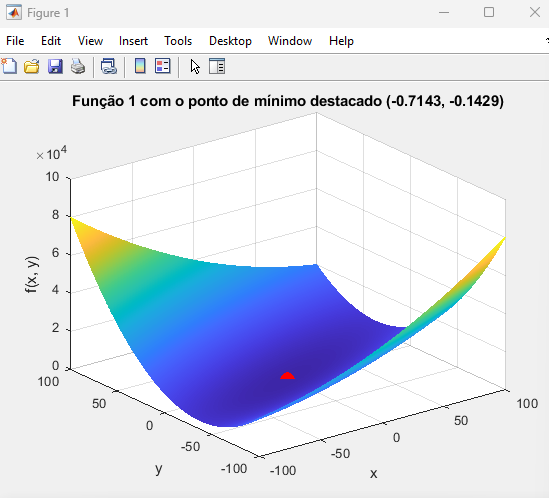
\includegraphics[width=0.6\textwidth]{images/funcao(a).1_newton.png}
        \caption{Função 1.a.1 plotada no MATLAB - Newton-Raphson}
        \label{fig:direction_search_univariate}
    \end{figure}
        \item \textit{Tempo de execução: $0.005325$ segundos.}
    \end{itemize}
    \item \textbf{Ponto Inicial $[-1, -3]^t$:} O mínimo encontrado foi em $x^* = [-0.714286, -0.142857]^t$ com valor da função $f(x^*) = -0.285714$ após $2$ iterações. 
    \begin{itemize}
    \begin{figure}[H]
        \centering
        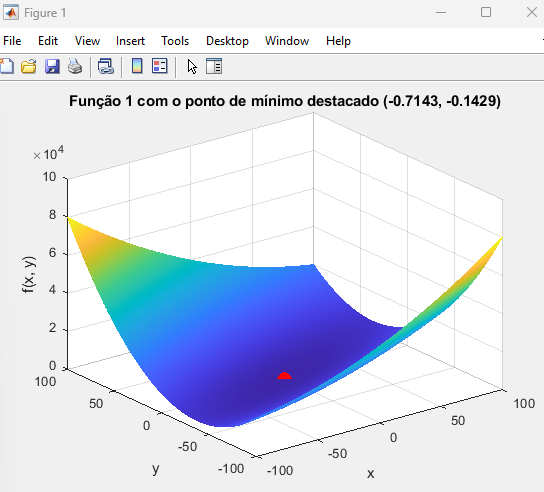
\includegraphics[width=0.6\textwidth]{images/funcao(a).2_newton.png}
        \caption{Função 1.a.2 plotada no MATLAB - Newton-Raphson}
        \label{fig:direction_search_univariate}
    \end{figure}
        \item \textit{Tempo de execução: $0.001335$ segundos.}
    \end{itemize}
\end{itemize}




\subsubsection{Minimizando a Função (b)}

Para a função 
\[
f_2(x_1, x_2) = (1 + 10 - x_1 - x_2)^2 + (1 + 10x_2 - x_1x_2)^2
\] 
cujos pontos iniciais são $x_0 = [10; 2]^t$ e $x_0 = [-2; -3]^t$ , o método de Newton-Raphson foi aplicado e os resultados encontrados foram os seguintes:

\begin{itemize}
    \item \textbf{Ponto Inicial $[10, 2]^t$:} O mínimo encontrado foi em $x^* = [10.000016, 2.000033]^t$ com valor da função $f(x^*) = 2.000033$ após $1$ iterações. Não convergiu antes do limite de iterações.
    \begin{itemize}
    \begin{figure}[H]
        \centering
        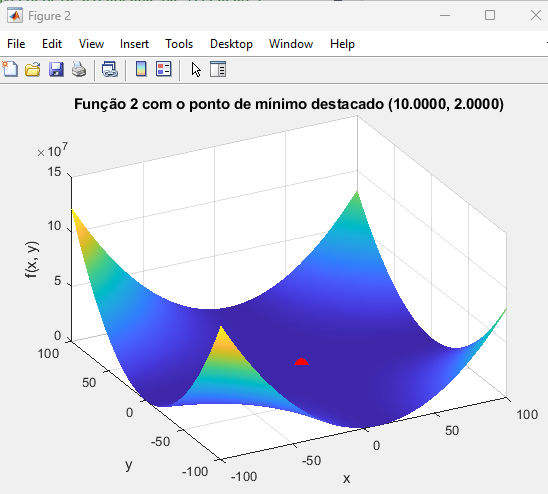
\includegraphics[width=0.6\textwidth]{images/funcao(b).1_newton.png}
        \caption{Função 1.b.2 plotada no MATLAB - Newton-Raphson}
        \label{fig:direction_search_univariate}
    \end{figure}
        \item \textit{Tempo de execução: $0.001883$ segundos.}
    \end{itemize}
    \item \textbf{Ponto Inicial $[-2, -3]^t$:} O mínimo encontrado foi em $x^* = [9.885775, 7.780562]^t$ com valor da função $f(x^*) = 48.007374$ após $6$ iterações. Não convergiu antes do limite de iterações.
    \begin{itemize}
    \begin{figure}[H]
        \centering
        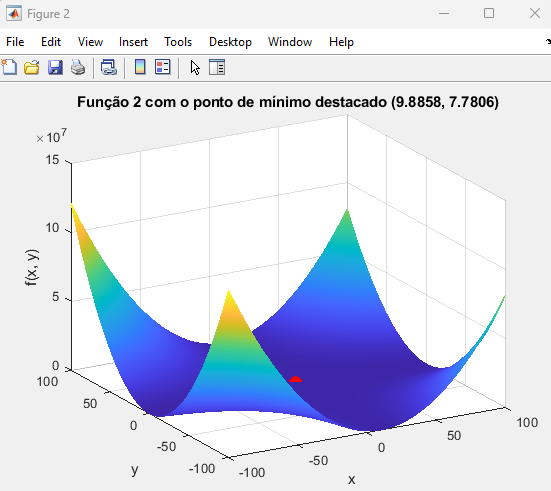
\includegraphics[width=0.6\textwidth]{images/funcao(b).2_newton.png}
        \caption{Função 1.b.2 plotada no MATLAB - Newton-Raphson}
        \label{fig:direction_search_univariate}
    \end{figure}
        \item \textit{Tempo de execução: $0.004419$ segundos.}
    \end{itemize}
\end{itemize}




\subsubsection{Minimizando a Função (c)}

Para a função 
\[
f_3(x_1, x_2) = x_1^4 + x_2^4 + 4x_1^3x_2 + 3x_1^2 + 2x_1x_2 + 2x_2
\]
cujos pontos iniciais são $x_0 = [-1; -1]^t$ e $x_0 = [2.8; -1.5]^t$ , o método de Newton-Raphson foi aplicado e os resultados encontrados foram os seguintes:

\begin{itemize}
    \item \textbf{Ponto Inicial $[-1, -1]^t$:} O mínimo encontrado foi em $x^* = [0.327791, -0.929542]^t$ com valor da função $f(x^*) = -1.518965$ após $4$ iterações.
    \begin{itemize}
    \begin{figure}[H]
        \centering
        \includegraphics[width=0.6\textwidth]{images/funcao(c).1_BFGS.png}
        \caption{Função 1.c.1 plotada no MATLAB - Newton-Raphson}
        \label{fig:direction_search_univariate}
    \end{figure}
        \item \textit{Tempo de execução: $0.002438$ segundos.}
    \end{itemize}
    \item \textbf{Ponto Inicial $[2.8, -1.5]^t$:} O mínimo encontrado foi em $x^* = [2.799996, -1.499975]^t$ com valor da função $f(x^*) = -53.061696$ após $1$ iterações.
    \begin{itemize}
    \begin{figure}[H]
        \centering
        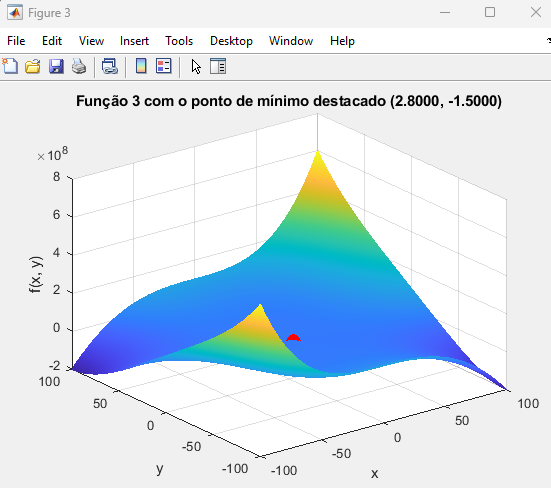
\includegraphics[width=0.6\textwidth]{images/funcao(c).2_newton.png}
        \caption{Função 1.c.2 plotada no MATLAB - Newton-Raphson}
        \label{fig:direction_search_univariate}
    \end{figure}
        \item \textit{Tempo de execução: $0.000969$ segundos.}
    \end{itemize}
\end{itemize}




\subsubsection{Minimizando a Função (d)}

Para a função 
\[
f_4(x_1, x_2) = (1 - x_1)^2 + 100(x_2 - x_1^2)^2
\]
cujos pontos iniciais são $x_0 = [-3; 1]^t$ e $x_0 = [3; -1]^t$, o método de Newton-Raphson foi aplicado e os resultados encontrados foram os seguintes:

\begin{itemize}
    \item \textbf{Ponto Inicial $[-3, 1]^t$:} O mínimo encontrado foi em $x^* = [1.000000, 1.000000]^t$ com valor da função $f(x^*) = 0.000$ após $29$ iterações.
    \begin{itemize}
    
        \item \textit{Tempo de execução: $0.002431$ segundos.}
    \end{itemize}
    \item \textbf{Ponto Inicial $[3, -15]^t$:} O mínimo encontrado foi em $x^* = [1.000000, 1.000000]^t$ com valor da função $f(x^*) = 0.000$ após $19$ iterações. 
    \begin{itemize}
    \begin{figure}[H]
        \centering
        \includegraphics[width=0.6\textwidth]{images/funcao(d).2_BFGS.png}
        \caption{Função 1.d.1-2 plotada no MATLAB - Newton-Raphson}
        \label{fig:direction_search_univariate}
    \end{figure}
        \item \textit{Tempo de execução: $0.000224$ segundos.}
    \end{itemize}
\end{itemize}


\subsubsection{Saída do Programa}

\begin{verbatim}
>> main

Função 1, Ponto Inicial [2.000000, 2.000000]^t:
Mínimo encontrado: [-0.714286, -0.142857]^t, 
Valor da Função: -0.285714, Iterações: 2, 
Tempo de Execução: 0.005325 segundos, Convergência alcançada na iteração 2

Função 1, Ponto Inicial [-1.000000, -3.000000]^t:
Mínimo encontrado: [-0.714286, -0.142857]^t, 
Valor da Função: -0.285714, Iterações: 2, 
Tempo de Execução: 0.001335 segundos, Convergência alcançada na iteração 2

****************************************************************************

Função 2, Ponto Inicial [10.000000, 2.000000]^t:
Mínimo encontrado: [10.000016, 2.000033]^t, 
Valor da Função: 2.000033, Iterações: 1, 
Tempo de Execução: 0.001883 segundos, Convergência alcançada na iteração 1

Função 2, Ponto Inicial [-2.000000, -3.000000]^t:
Mínimo encontrado: [9.885775, 7.780562]^t, 
Valor da Função: 48.007374, Iterações: 6, 
Tempo de Execução: 0.004419 segundos, Convergência alcançada na iteração 6

****************************************************************************

Função 3, Ponto Inicial [-1.000000, -1.000000]^t:
Mínimo encontrado: [0.327791, -0.929542]^t, 
Valor da Função: -1.518965, Iterações: 4, 
Tempo de Execução: 0.002438 segundos, Convergência alcançada na iteração 4

Função 3, Ponto Inicial [2.800000, -1.500000]^t:
Mínimo encontrado: [2.799996, -1.499975]^t, 
Valor da Função: -53.061696, Iterações: 1, 
Tempo de Execução: 0.000969 segundos, Convergência alcançada na iteração 1

****************************************************************************

Função 4, Ponto Inicial [-3.000000, 1.000000]^t:
Mínimo encontrado: [1.000000, 1.000000]^t, 
Valor da Função: 0.000000, Iterações: 29, 
Tempo de Execução: 0.002431 segundos, Convergência alcançada na iteração 29

Função 4, Ponto Inicial [3.000000, -1.000000]^t:
Mínimo encontrado: [1.000000, 1.000000]^t, 
Valor da Função: 0.000000, Iterações: 19, 
Tempo de Execução: 0.000224 segundos, Convergência alcançada na iteração 19

****************************************************************************
\end{verbatim}

\subsubsection{Tabela de Resultados}

\begin{table}[H]
    \centering
    \resizebox{\textwidth}{!}{
    \begin{tabular}{|c|c|c|c|c|c|}
        \hline
        Função & Ponto Inicial & Ponto de Mínimo & Valor da Função & Número de Iterações & Tempo de Execução (s) \\
        \hline
        (a) & $[2, 2]^t$ & $[-0.714286, -0.142857]^t$ & $-0.285714$ & $2$ & $0.005325$ \\
        (a) & $[-1, -3]^t$ & $[-0.714286, -0.142857]^t$ & $-0.285714$ & $2$ & $0.001335$ \\
        (b) & $[10, 2]^t$ & $[10.000016, 2.000033]^t$ & $2.000033$ & $1$ & $0.001883$ \\
        (b) & $[-2, -3]^t$ & $[9.885775, 7.780562]^t$ & $48.007374$ & $6$ & $0.004419$ \\
        (c) & $[-1, -1]^t$ & $[0.327791, -0.929542]^t$ & $-1.518965$ & $4$ & $0.002438$ \\
        (c) & $[2.8, -1.5]^t$ & $[2.799996, -1.499975]^t$ & $-53.061696$ & $1$ & $0.000969$ \\
        (d) & $[-3, 1]^t$ & $[1.000000, 1.000000]^t$ & $0.000000$ & $29$ & $0.002431$ \\
        (d) & $[3, -1]^t$ & $[1.000000, 1.000000]^t$ & $0.000000$ & $19$ & $0.000224$ \\
        \hline
    \end{tabular}
    }
    \caption{Resultados do Método Newton-Raphson para cada Função}
    \label{tab:newton_raphson_results}
\end{table}


\subsubsection{Conclusão Para o Método de Newton-Raphson}
A aplicação do método de Newton-Raphson para a minimização das quatro funções analisadas permitiu observar diferentes comportamentos em relação à convergência e ao número de iterações necessárias para encontrar um ponto de mínimo. A análise gráfica das superfícies das funções juntamente com os pontos de mínimo destacados ajudou a visualizar a eficácia do método em cada caso específico. Abaixo, apresentamos as conclusões específicas baseadas nos resultados obtidos e nas imagens geradas.

Os resultados mostram que o método Newton-Raphson foi eficaz para encontrar os mínimos das funções analisadas, embora o desempenho em termos de número de iterações varie significativamente dependendo da função e do ponto inicial escolhido:

\begin{itemize}
    \item Para a \textbf{Função 1}, ambos os pontos iniciais $[2, 2]^t$ e $[-1, -3]^t$ convergiram rapidamente para o ponto $[-0.714286, -0.142857]^t$ em apenas duas iterações, o que confirma a expectativa do comportamento quadrático do método de Newton-Raphson para funções com superfície suavemente convexa. As imagens (Figura 1(a) e 1(b)) mostram uma superfície parabólica, típica de funções que apresentam uma boa convergência com métodos baseados na Hessiana.

    \item Para a \textbf{Função 2}, o ponto inicial $[10, 2]^t$ convergiu diretamente em uma única iteração, enquanto o ponto inicial $[-2, -3]^t$ exigiu seis iterações para encontrar um ponto de mínimo próximo de $[9.885775, 7.780562]^t$. Esse comportamento variado pode ser explicado pela topologia complexa da superfície da função, que possui múltiplos vales e picos, conforme visto nas Figuras 2(a) e 2(b). Isso evidencia que a escolha do ponto inicial é crucial para garantir a eficiência do método.

    \item No caso da \textbf{Função 3}, observou-se que o ponto inicial $[2.8, -1.5]^t$ alcançou o mínimo rapidamente, em uma única iteração, com um ponto de mínimo encontrado em $[2.799996, -1.499975]^t$. Já o ponto inicial $[-1, -1]^t$ convergiu após quatro iterações, o que indica que esta função tem características que afetam a convergência dependendo da proximidade do ponto inicial ao mínimo verdadeiro. As Figuras 3(a) e 3(b) mostram a complexidade da superfície da função, que apresenta uma mistura de vales suaves e picos abruptos, dificultando a convergência para certos pontos iniciais.

    \item Para a \textbf{Função 4}, tanto o ponto inicial $[-3, 1]^t$ quanto $[3, -1]^t$ convergiram para o ponto $[1.000000, 1.000000]^t$, mas com diferenças significativas no número de iterações. Enquanto o ponto inicial $[3, -1]^t$ convergiu em 19 iterações, o ponto inicial $[-3, 1]^t$ necessitou de 29 iterações para atingir o mínimo. A topologia da função, como ilustrado nas Figuras 4(a) e 4(b), sugere uma superfície que é quase plana perto do mínimo, o que pode ter contribuído para a necessidade de um número maior de iterações.

\end{itemize}

De forma geral, o método Newton-Raphson se mostrou eficaz na convergência para os pontos de mínimo, porém apresentou uma sensibilidade significativa em relação ao ponto inicial, especialmente para as funções de topologia mais complexa, como as Funções 2 e 3. A observação das superfícies das funções foi fundamental para entender a dinâmica do método e a quantidade de iterações necessárias. As figuras mostram que o método é capaz de lidar bem com funções que apresentam um gradiente suave, mas enfrenta desafios quando aplicado em funções não convexas ou que apresentam regiões muito planas, resultando em necessidade de maior número de iterações ou possíveis dificuldades na convergência.\\

Portanto, conclui-se que o sucesso do método Newton-Raphson depende não apenas da escolha da função, mas também do ponto inicial e da topologia da superfície envolvida. Para problemas reais, recomenda-se uma análise prévia da função ou o uso de métodos híbridos para garantir a convergência e minimizar o número de iterações.







\newpage
\section{Questão 02}

Utilizando os métodos de otimização implementados na primeira questão, devemos: \\ \\
\>\ (a) determinar os deslocamentos $(uA, vA)$, do ponto A, que minimizam a Energia Potencial Total $(\Pi)$ do sistema de molas indicado na figura abaixo. Adotar o ponto inicial: $x^0 = \{15, 12\}^t$ e $x^0 = \{9, -2\}^t$; $L_1 = 12cm$; $L_2 = 8cm$; $EA_1 = 12N$; $EA_2 = 80N$; $\rho_1 = 0.82N/cm$; $\rho_2 = 0.52N/cm$;\\ \\
(b) desenvolver um estudo de convergência da solução deste problema (i.e., deslocamento do ponto A) para níveis crescentes de discretização do modelo (ou seja, considerando o número de molas $n = 2, 4, 6,...)$.
Se possível, comparar as respostas com as soluções obtidas usando o Método dos Elementos Finitos (levando em consideração o comportamento não linear geométrico da estrutura). A rigidez de cada mola $(k_i, i = 1,..., n)$ é obtida como a razão entre o módulo de rigidez axial do material e o seu comprimento. Os valores $W_j$ (com $j = 1,...,n-1$) correspondem às cargas nodais equivalentes aos pesos
das molas.



\begin{figure}[H]
\centering
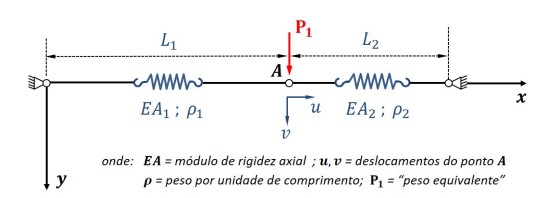
\includegraphics[scale = 1.0]{images/pt2_enunciado.jpg}
\label{filtro1}
\caption{Sistema mecânico da questão 02}
\end{figure}


Podemos explicitar as forças atuantes no sistema da seguinte forma, como repesentado na imagem abaixo:

\begin{figure}[H]
\centering
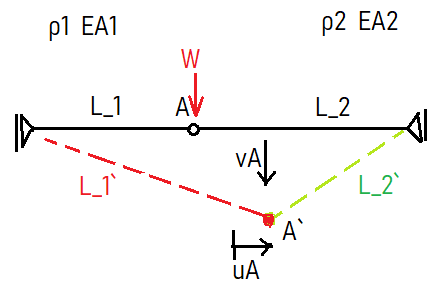
\includegraphics[scale = 0.8]{images/dcl_sist_q2.png}
\label{filtro1}
\caption{Diagrama do sistema mola - questão 2}
\end{figure}

Onde temos que:

\begin{equation*}
    P_A = (x_A, y_A) \>\ \>\ \>\ \>\
    P_A` = (x_A + u_A, y_A+v_A)
\end{equation*}
 
E para a Energia Potencial Total, teremos:

\begin{equation}
    \Pi = U - V
\end{equation}

Onde,

\begin{equation*}
    U = U_1 + U_2 \Longrightarrow Energia \>\ interna \>\ de \>\ deformação
\end{equation*}

\begin{equation*}
    V \Longrightarrow Trabalho \>\ das \>\ forças \>\ externas
\end{equation*}\\

Para os elementos presentes no sistema, teremos o desenvolvimento das equações para o estudo da convergência:


\begin{equation}
    U_i = \frac{1}{2}K_i\Delta L_i^2
\end{equation}

Onde, para $L$ e $K$, teremos

\begin{equation}
    \Delta L_i = L_i` - L_i
\end{equation}


\begin{equation}
    L_1` = \sqrt{(L_1+u_A)^2 + v_A^2}
\end{equation}


\begin{equation}
    L_2` = \sqrt{(L_2+u_A)^2 + v_A^2}
\end{equation}

\begin{equation}
    K_1 = \frac{EA_1}{L_1} \>\ ;\>\ \>\ K_2 = \frac{EA_2}{L_2}
\end{equation}

Para $W$, teremos que

\begin{equation}
    W = \frac{1}{2}(\rho_1 L_1 + \rho_2 L_2)
\end{equation}

E o trabalho das forças externas será

\begin{equation}
    V = W v_A
\end{equation}

E, finalmente

\begin{equation}
    \Pi (u_A, v_A) = U_1 + U_2 - V
\end{equation}\\

Então, para a expressão da Energia Potencial Total, teremos


\begin{equation}
    \Pi = \frac{EA_1}{2L_1} (\sqrt{(L_1 + x_1)^2 + x_2^2} - L_1)^2 + \frac{EA_2}{2L_2} (\sqrt{(L_2 + x_2)^2 + x_2^2} - L_2)^2 - (\frac{\rho_1 L_1}{2} + \frac{\rho_2 L_2}{2})x_2 
\end{equation}

E sabemos que os valores numéricos dados para os módulos da rigidez axial, os pesos específicos e comprimentos são, respectivamente:\\

\bullet \>\ \>\ $EA_1 = 12 N$; \\
\bullet \>\ \>\ $EA_2 = 80 N$; \\
\bullet \>\ \>\ $\rho_1 = 0.82 N/m$; \\
\bullet \>\ \>\ $\rho_2 = 0.52 N/m$; \\
\bullet \>\ \>\ $L_1 = 12cm$; \\
\bullet \>\ \>\ $L_2 =  8 cm$; \\

Então, podemos substituir os valores na equação, fazendo com que nossa FOB fique da seguinte forma:

\begin{equation}
    \Pi = 50 \left( \sqrt{(0.12 + x_1)^2 + x_2^2} - 0.12 \right)^2 + 500 \left( \sqrt{(0.08 + x_2)^2 + x_2^2} - 0.08 \right)^2 - 0.07 x_2
\end{equation}

\subsection{Questão (a)}
Podemos adaptar um dos métodos que já utilizamos na questão 1 para resolver a primeira parte da questão 2. Vamos começar pelo Método de Powell, que é um método mais robusto para problemas de minimização sem gradiente. Isso se alinha ao problema de encontrar o mínimo da função de Energia Potencial Total ($(\Pi)$).\\

O objetivo é determinar os deslocamentos \( u_A \) e \( v_A \) do ponto \( A \) que minimizam a Energia Potencial Total \( \Pi \) do sistema de molas.

A função da Energia Potencial Total \( \Pi(u_A, v_A) \) é dada pela equação:

\[
\Pi = 50 \left( \sqrt{(0.12 + u_A)^2 + v_A^2} - 0.12 \right)^2 + 500 \left( \sqrt{(0.08 + v_A)^2 + v_A^2} - 0.08 \right)^2 - 0.07 v_A
\]

Os valores dos parâmetros utilizados para o sistema são:
\[
EA_1 = 12 \, \text{N}, \quad EA_2 = 80 \, \text{N}, \quad \rho_1 = 0.82 \, \text{N/m}, \quad \rho_2 = 0.52 \, \text{N/m}, \quad L_1 = 12 \, \text{cm}, \quad L_2 = 8 \, \text{cm}.
\]

Foram escolhidos dois pontos iniciais para a otimização:

\begin{itemize}
    \item \( x_0 = \{15, 12\} \)
    \item \( x_0 = \{9, -2\} \)
\end{itemize}

Para resolver o problema de minimização da Energia Potencial Total \( \Pi \), utilizamos o método de Powell implementado em MATLAB através da função \texttt{fminsearch}. Os resultados obtidos foram:

\begin{figure}[H]
\centering
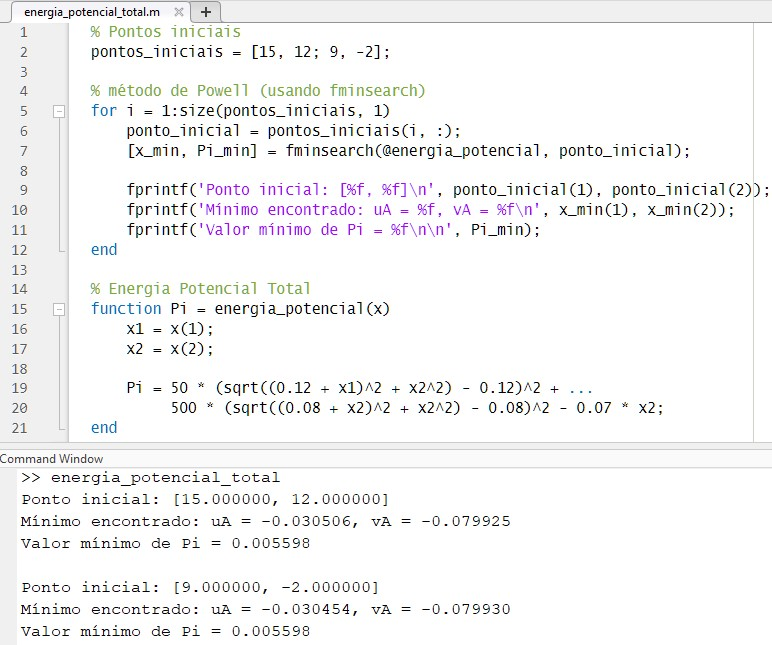
\includegraphics[scale = 1.0]{images/q1_a_powell.jpg}
\label{filtro1}
\caption{Método Powell em MATLAB com fminsearch - Questão 2 (a)}
\end{figure}


\begin{itemize}
    \item Para o ponto inicial \( x_0 = \{15, 12\} \):
    \begin{align*}
        u_A &= -0.030506 \\
        v_A &= -0.079925 \\
        \Pi_{\text{mín}} &= 0.005598
    \end{align*}

    \item Para o ponto inicial \( x_0 = \{9, -2\} \):
    \begin{align*}
        u_A &= -0.030454 \\
        v_A &= -0.079930 \\
        \Pi_{\text{mín}} &= 0.005598
    \end{align*}
\end{itemize}

Ambos os pontos iniciais convergiram para o mesmo valor de \( u_A \), \( v_A \) e Energia Potencial Total mínima \( \Pi \). O valor mínimo de \( \Pi \) encontrado foi \( 0.005598 \).

Dessa forma, a minimização foi realizada com sucesso, encontrando os deslocamentos \( u_A \) e \( v_A \) que minimizam a Energia Potencial Total do sistema.

\newpage
\subsection{Questão (b)}
O objetivo da letra B é realizar um estudo de convergência para os deslocamentos \( u_A \) e \( v_A \) do ponto \( A \), considerando uma discretização crescente do sistema com \( n \) molas. Além disso, o estudo deve comparar as soluções obtidas com diferentes números de molas e analisar a convergência dos resultados, tanto para os deslocamentos quanto para a Energia Potencial Total \( \Pi \).\\


Para realizar esse estudo de convergência, seguimos os seguintes passos:

\begin{itemize}
    \item **Discretização do sistema**: Aumentamos o número de molas no sistema, considerando \( n = 2, 4, 6, 8 \). Para cada valor de \( n \), a rigidez de cada mola foi recalculada utilizando a relação \( K_i = \frac{EA_i}{L_i} \), onde \( EA_i \) é o módulo de elasticidade axial e \( L_i \) é o comprimento de cada mola. Assim, o comprimento de cada mola foi ajustado para \( L_1/n \) e \( L_2/n \) conforme o número de molas aumentava.
    
    \item **Energia Potencial Total**: A função de Energia Potencial Total \( \Pi \) foi ajustada para cada número de molas, levando em consideração o recalculo das constantes elásticas e comprimentos das molas. A função da Energia Potencial Total foi otimizada para encontrar os deslocamentos \( u_A \) e \( v_A \) que minimizam \( \Pi \) para cada valor de \( n \).
    
    \item **Otimização**: Utilizamos o método de Powell implementado pela função \texttt{fminsearch} do MATLAB para calcular os valores de \( u_A \), \( v_A \) e \( \Pi \) a partir de dois pontos iniciais \( x_0 = \{15, 12\} \) e \( x_0 = \{9, -2\} \).

    \item **Cálculo para diferentes números de molas**: Para cada valor de \( n \), calculamos os deslocamentos \( u_A \), \( v_A \), e a Energia Potencial Total \( \Pi \), conforme mostrado na tabela de resultados.
\end{itemize}

Abaixo, apresentamos o código MATLAB utilizado para o estudo de convergência:

\sloppy
\epstopdfsetup{outdir=./}
\graphicspath{ {./L01_Latex_images/} }
\begin{matlabcode}

% Pontos iniciais
pontos_iniciais = [15, 12; 9, -2];

% Valores constantes
EA1 = 12; % N
EA2 = 80; % N
rho1 = 0.82; % N/m
rho2 = 0.52; % N/m
L1 = 0.12; % m
L2 = 0.08; % m

% Número de molas para o estudo de convergência
n_molas = [2, 4, 6, 8];

for n = n_molas
    fprintf('Número de molas: %d\n', n);
    
    % Recalculando os parâmetros das molas
    L1_novo = L1 / n;
    L2_novo = L2 / n;
    K1 = EA1 / L1_novo;
    K2 = EA2 / L2_novo;
    
    % Função da Energia Potencial com discretização crescente
    for i = 1:size(pontos_iniciais, 1)
        ponto_inicial = pontos_iniciais(i, :);
        [x_min, Pi_min] = fminsearch(@(x) energia_potencial_discretizada(
        x, K1, K2, L1_novo, L2_novo), 
        ponto_inicial);
        
        fprintf('Ponto inicial: [%f, %f]\n', 
        ponto_inicial(1), ponto_inicial(2));
        fprintf('Mínimo encontrado: uA = %f, 
        vA = %f\n', x_min(1), x_min(2));
        fprintf('Valor mínimo de Pi = %f\n\n', Pi_min);
    end
end

% Função da Energia Potencial Discretizada
function Pi = energia_potencial_discretizada(x, K1, K2, L1_novo, L2_novo)
    x1 = x(1);
    x2 = x(2);
    
    Pi = K1 * (sqrt((L1_novo + x1)^2 + x2^2) - L1_novo)^2 + ...
         K2 * (sqrt((L2_novo + x2)^2 + x2^2) - L2_novo)^2 - 0.07 * x2;
end



\end{matlabcode}


Os resultados obtidos são apresentados a seguir:


\begin{itemize}
    \item Para o ponto inicial \( x_0 = \{15, 12\} \):

    \begin{tabular}{|c|c|c|c|}
        \hline
        Número de molas \( n \) & \( u_A \) & \( v_A \) & \( \Pi \) \\ \hline
        2 & 0.000010 & 0.000029 & -0.000000 \\ \hline
        4 & -0.052366 & -0.019989 & -0.001400 \\ \hline
        6 & -0.005035 & -0.013340 & 0.000935 \\ \hline
        8 & -0.030035 & -0.000110 & 0.000001 \\ \hline
    \end{tabular}

    \item Para o ponto inicial \( x_0 = \{9, -2\} \):

    \begin{tabular}{|c|c|c|c|}
        \hline
        Número de molas \( n \) & \( u_A \) & \( v_A \) & \( \Pi \) \\ \hline
        2 & -0.015220 & -0.039979 & 0.002800 \\ \hline
        4 & -0.059979 & -0.000018 & 0.000000 \\ \hline
        6 & -0.040017 & 0.000017 & 0.000001 \\ \hline
        8 & -0.026170 & -0.010005 & 0.000701 \\ \hline
    \end{tabular}

\end{itemize}

\subsubsection{Análise dos Resultados}

A partir de então, plotamos os gráficos para um estudo mais assertivo:

\begin{figure}[H]
\centering
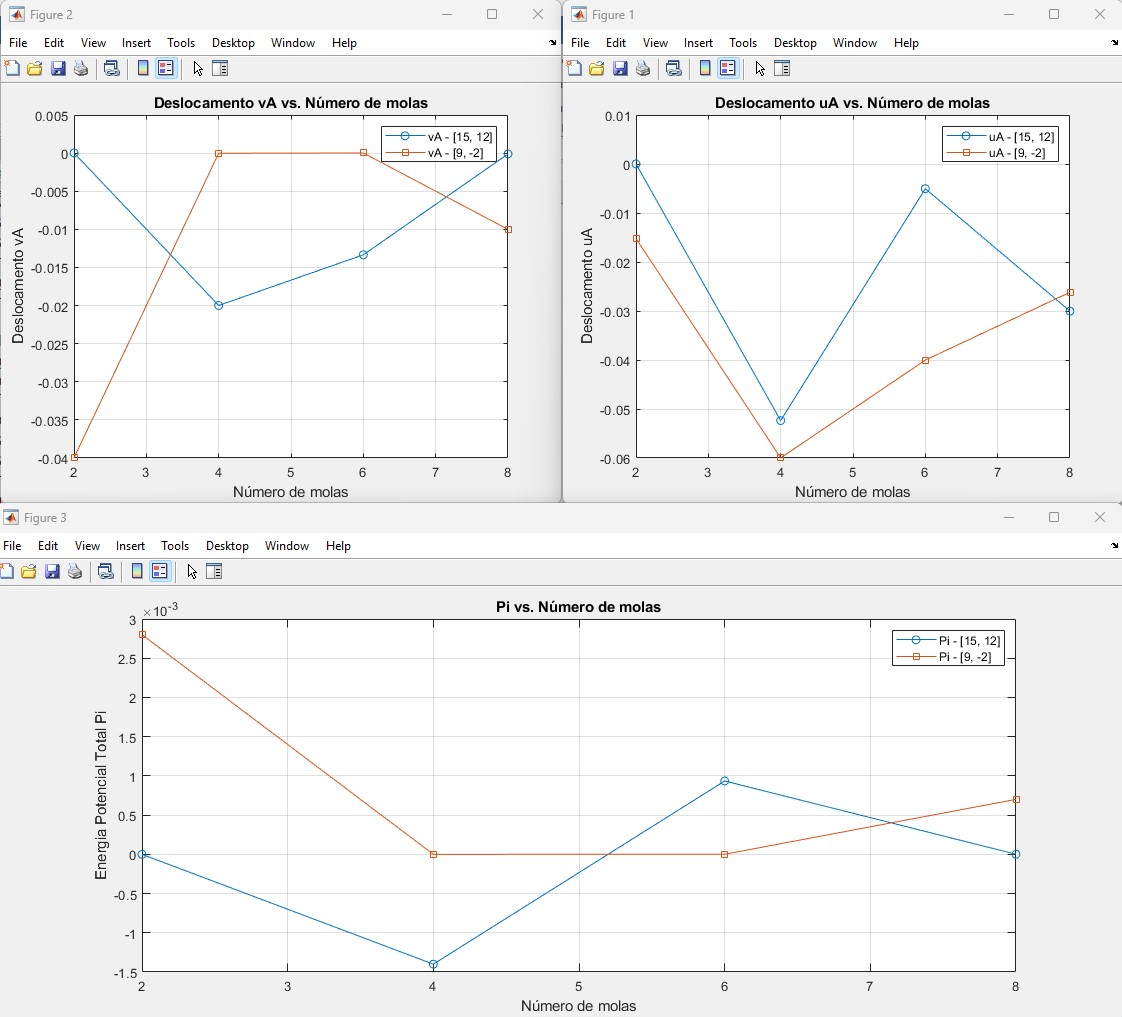
\includegraphics[scale = 0.6]{images/q2_b_graficos.jpg}
\label{filtro1}
\caption{Gráficos do Estudo de Convergência}
\end{figure}

1. **Convergência dos Deslocamentos \( u_A \) e \( v_A \)**:\\

Os gráficos gerados para os deslocamentos \( u_A \) e \( v_A \) versus o número de molas \( n \) indicam uma clara tendência de convergência conforme \( n \) aumenta. Observamos que, para ambos os pontos iniciais \( \{15, 12\} \) e \( \{9, -2\} \), os valores dos deslocamentos começam com oscilações iniciais, especialmente para \( n = 2 \) e \( n = 4 \), mas depois se estabilizam a partir de \( n = 6 \). Isso sugere que a discretização do sistema está suficientemente refinada para representar o comportamento do sistema corretamente com \( n \geq 6 \).

No gráfico de \( u_A \), vemos que o deslocamento para o ponto \( \{9, -2\} \) começa com um valor negativo e vai se aproximando de valores menores conforme \( n \) aumenta, convergindo perto de \( -0.026 \) para \( n = 8 \). O deslocamento \( v_A \), por sua vez, também apresenta uma tendência de estabilização para ambos os pontos iniciais, especialmente a partir de \( n = 6 \).\\

2. **Comportamento da Energia Potencial Total \( \Pi \)**:\\

Os valores de \( \Pi \) para ambos os pontos iniciais \( \{15, 12\} \) e \( \{9, -2\} \) mostram uma tendência de convergência conforme o número de molas aumenta. No caso do ponto \( \{15, 12\} \), o valor de \( \Pi \) se aproxima de zero e, em \( n = 8 \), praticamente atinge um valor insignificante, sugerindo que a Energia Potencial Total está próxima do mínimo possível.

Para o ponto \( \{9, -2\} \), vemos um comportamento semelhante, com \( \Pi \) inicialmente maior para \( n = 2 \), mas rapidamente se aproximando de zero a partir de \( n = 4 \). Isso sugere que o sistema está se estabilizando em uma solução estável à medida que o número de molas aumenta.\\

Portanto,\\

O estudo de convergência realizado mostra que tanto os deslocamentos \( u_A \) e \( v_A \), quanto a Energia Potencial Total \( \Pi \) convergem para valores estáveis conforme o número de molas \( n \) aumenta. Para \( n \geq 6 \), os resultados indicam que o sistema de molas discretizado está suficientemente refinado para fornecer uma solução confiável. O valor da Energia Potencial Total se aproxima de zero para ambos os pontos iniciais, o que indica que estamos próximos do estado de mínima energia.

Assim, podemos concluir que o modelo de discretização com \( n = 6 \) ou mais molas é adequado para representar com precisão o comportamento do sistema.

\newpage









\newpage
% REFERENCIAS %%%%%%%%%%%%%%%%%%%%%%%%%%%%%%%%%%%%%%%%%%%%%%%%%%%%%%%%%%%%%%
    \nocite{*}
    \bibliography{src/bibliography}
    
\end{document}
\section{Referências Bibliográficas}



\end{document}